%----------------------------------------------------------------
%
%  File    :  thesis.tex
%
%  Author  :  Keith Andrews, ISDS, TU Graz, Austria
%
%  Created :  30 Jul 1997
% 
%  Changed :  22 Jan 2021
%
%----------------------------------------------------------------

\documentclass[11pt]{book}
\usepackage[
  a4paper,
  twoside,
  top=5mm,                % top margin
  bottom=7mm,             % bottom margin
  inner=20mm,             % inner margin (next to binding)
  outer=20mm,             % outer margin (opposite binding)
  bindingoffset=10mm,     % on binding side
  includeheadfoot,        % include head(er) and foot(er)
  headheight=10mm,        % height of header
  headsep=15mm,           % sep between header and text body
  footskip=15mm,          % sep between body and baseline of footer
  footnotesep = 10mm plus 2mm minus 0mm  % bottom of body to top of footnote
]{geometry}
% A4 paper is w=210m, h=297mm


\newcommand{\thisdate}{22 Jan 2021}  % date of this version
\newcommand{\thisyear}{2021}         % year of this version


\newcommand{\fullh}{24cm}         % height of figures for 1 per page
\newcommand{\halfh}{9.5cm}        % height of figures for 2 per page
\newcommand{\thirdh}{6cm}         % height of figures for 3 per page


\setlength{\parindent}{1em}       % less indentation
\setlength{\parskip}{1.5ex plus 0.3ex minus 0.3ex}  % vert. space before para


% \tolerance is set by LaTeX to 200
% \sloppy sets \tolerance = 9999
% which allows LaTeX more tolerance in adding word spacing

% \sloppy
% \fussy
% \tolerance = 1000

\tolerance=400 
% makes some lines with lots of white space, but      
% tends to prevent words from sticking out in the margin



\setcounter{secnumdepth}{3}     % lowest section level still numbered
\setcounter{tocdepth}{2}        % lowest section level entered in ToC




\usepackage[T1]{fontenc}        % 8-bit output chars (must be before inputenx)
\usepackage[utf8]{inputenx}     % input char encoding

\usepackage[english,austrian,british]{babel}

\usepackage{newtxtext}          % newer times fonts
\usepackage{newtxmath}

\usepackage{relsize}            % relative font sizes \smaller \larger
\usepackage{float}              % H for float placement
\usepackage{setspace}           % adjust line spacing

\usepackage{textcomp}           % symbols such as \texttimes and \texteuro
\usepackage{latexsym}
\usepackage{fontawesome}        % fontawesome symbols

\usepackage{siunitx}            % prettier number formatting
\sisetup{%
  group-separator={,},
  group-minimum-digits=4,
}
\usepackage[super]{nth}         % 1st, 2nd, 3rd, etc.

\usepackage{xspace}
\usepackage{xstring}            % string manipulation macros
\usepackage{xparse}             % commands with optional arguments
\usepackage{etoolbox}           % for \newrobustcmd
\usepackage{makecmds}           % for \makecommand
\usepackage{calc}               % for math calculations


\usepackage[svgnames,table,xcdraw]{xcolor}
\definecolor{darkgreen}{rgb}{0.0,0.2,0.0}
\definecolor{darkblue}{rgb}{0.0,0.0,0.2}
\definecolor{darkred}{rgb}{0.2,0.0,0.0}
\definecolor{verylightgrey}{gray}{0.95}
\definecolor{lightgrey}{gray}{0.9}
\definecolor{grey}{gray}{0.7}
\definecolor{black}{gray}{0.0}


\usepackage{longtable}
\usepackage{multirow}
\usepackage{tabularx}

\usepackage{verbdef}            % define robust verb strings
\usepackage{verbatim}
\usepackage{comment}



% better lists
\usepackage{enumitem}

\setlist{
  topsep=0pt,
  partopsep=0pt,
  parsep=0.6ex,
  itemsep=1.2ex,
  left=\parindent .. 2\parindent,    % bullet .. start ot text
}

\setlist[description]{
  style=sameline,
}




\usepackage{listings}                 % for listings of source code

\makeatletter
\newlength{\numwidth}%
\setlength{\numwidth}{\widthof{\normalfont{\lst@numberstyle{99}}}}% Up to 2-digit (99) line numbers
\def\lst@PlaceNumber{%
  \makebox[\numwidth+1em][l]{%
    \makebox[\numwidth][r]{\normalfont\lst@numberstyle{\thelstnumber}}%
  }%
}
\makeatother

% lstset strategy: define defaults here for
% all non-floating (displayed) listings
% floated listings override these settings later

\lstset{                              % set parameters for listings
  floatplacement=tp,                  % default float placement
  numberbychapter,
  inputencoding=utf8,
  language=,                          % empty = plain text
  tabsize=2,
  xleftmargin=2\parindent,
  xrightmargin=2\parindent,
  frame=none,
  framexleftmargin=0mm,
  rulesepcolor=\color{verylightgrey},
  numbers=none,
  numberstyle=\scriptsize,
  numbersep=2ex,
  breaklines,
  showtabs=false,
  showspaces=false,
  showstringspaces=false,
  %
  basicstyle=\small\ttfamily,
  keywordstyle=\color{black},
  identifierstyle=\color{black},
  commentstyle=\color{SteelBlue},
  stringstyle=\color{DarkOrange},
  %
  captionpos=b,
  abovecaptionskip=\abovecaptionskip,
  belowcaptionskip=\belowcaptionskip,
  extendedchars=true,
  literate=%
    { }{{~}}1
    {©}{{\textcopyright}}1
    {€}{{\texteuro}}1
    {Ö}{{\"O}}1
    {Ä}{{\"A}}1
    {Ü}{{\"U}}1
    {ß}{{\ss}}1
    {ö}{{\"o}}1
    {ä}{{\"a}}1
    {ü}{{\"u}}1,       % map some utf8 chars for listings
}


\lstdefinelanguage{biblatex}   % based on biblatex v 2.7a from 2013-07-14
{
  keywords={%
    @article,@book,@mvbook,@inbook,@bookinbook,@suppbook,%
    @booklet,@collection,@mvcollection,@incollection,@suppcollection,%
    @manual,@misc,@online,@patent,@periodical,@suppperiodical,%
    @proceedings,@mvproceedings,@inproceedings,@reference,@mvreference,%
    @inreference,@report,@set,@thesis,@unpublished,@xdata,%
    @conference,@electronic,@mastersthesis,@phdthesis,@techreport,@www,%
    @artwork,@audio,@bibnote,@commentary,@image,@jurisdiction,@legislation,%
    @legal,@letter,@movie,@music,@performance,@review,@software,%
    @standard,@video%
  },
  sensitive=false,
  comment=[l][\itshape]{@comment},
  morecomment=[l]{\%},
}

\lstdefinelanguage{CSS}
{
  alsoletter={-},
  morekeywords={%
  color,background,background-color,margin,padding,font,
  font-family,weight,%
  display,position,top,left,right,bottom,list,%
  style,border,size,white,space,min,width%
  },
  sensitive=false,
  morecomment=[l]{//},
  morecomment=[s]{/*}{*/},
  morestring=[b]",
}




\usepackage[compact,nobottomtitles,pagestyles,explicit]{titlesec}
% when using explicit, must explicitly include #1 for titlename

% nobottomtitles
% move section headings close to page bottom to next page
\renewcommand{\bottomtitlespace}{2cm}

% \chaptermark sets the value of \chaptertitle for later
% \@chapapp is defined as \chaptername outside the appendix,
% and as \appendixname within the appendix.
\makeatletter
\titleformat{\chapter}
[display]                                            % shape
{\chaptermark{\thechapter~~#1}\sffamily\bfseries}    % format
{\huge\@chapapp\ \thechapter}                        % label
{4ex}                                                % sep
{\Huge#1}                                            % before-code
\makeatother

\titleformat{name=\chapter,numberless}
[block]                                              % shape
{\chaptermark{#1}\sffamily\bfseries}                 % format
{}                                                   % label
{0ex}                                                % sep
{\Huge#1}                                            % before-code

\titleformat{\section}
{\normalfont\Large\sffamily\bfseries}{\thesection}{0.8em}{#1}

\titleformat{\subsection}
{\normalfont\large\sffamily\bfseries}{\thesubsection}{0.8em}{#1}

\titleformat{\subsubsection}
{\normalfont\normalsize\sffamily\bfseries}{\thesubsubsection}{0.8em}{#1}

\titleformat{\paragraph}[runin]
{\normalfont\normalsize\sffamily\bfseries}{\theparagraph}{0.8em}{#1}

\titleformat{\subparagraph}[runin]
{\normalfont\normalsize\sffamily\bfseries}{\thesubparagraph}{0.8em}{#1}


% vertical spacing before and after section titles
\titlespacing*{\section}
{0pt}{3.5ex plus 0.5ex minus 0.5ex}{0ex plus 0ex minus 0.2ex}

\titlespacing*{\subsection}
{0pt}{2.5ex plus 0.5ex minus 0.5ex}{0ex plus 0ex minus 0.2ex}

\titlespacing*{\subsubsection}
{0pt}{2ex plus 0.5ex minus 0.5ex}{0ex plus 0ex minus 0.2ex}

\titlespacing*{\paragraph}
{0pt}{1.5ex plus 0.3ex minus 0.3ex}{0ex plus 0ex minus 0.15ex}

\titlespacing*{\subparagraph}
{0pt}{1ex plus 0.2ex minus 0.2ex}{0ex plus 0ex minus 0.1ex}


% define page headings how I want them

\newpagestyle{main}[\small]{
% \addtolength\headheight{6.7pt}
% \headrule
\sethead%
[{\parbox[t]{0.3\textwidth}%                    % even left
  {\sffamily\thepage}}]
[]%                                             % even centre
[{\parbox[t]{0.6\textwidth}%                    % even right
  {\raggedleft\sffamily\chaptertitle}}]
{{\parbox[t]{0.6\textwidth}%                    % odd left
  {\sffamily\sectiontitle}}}%
{}%                                             % odd centre
{{\parbox[t]{0.3\textwidth}%                    % odd right
  {\raggedleft\sffamily\thepage}}}
}





\usepackage{titletoc}

% \contentsmargin{2.55em}

\titlecontents{chapter}%
[1.5em]%                         % left indent to entry text
{\addvspace{1em}\bfseries}%      % above-code per entry
{\contentslabel{1.5em}}%         % format for numbered entry
{\hspace*{-1.5em}}%              % format for unnumbered entry
{\hfill\contentspage}%           % [no dots] and page num per entry


% Note: \dottedcontents is short form of \titlecontents

\dottedcontents{section}%
[3.8em]%                         % left indent to entry text = 1.5 + 2.3
{}%                              % above-code per entry
{2.3em}%                         % label width
{1pc}%                           % space around the dots

\dottedcontents{subsection}%
[7.4em]%                         % left indent to entry text = 3.8 + 3.6
{}%                              % above-code per entry
{3.6em}%                         % label width
{1pc}%                           % space around the dots


\dottedcontents{figure}%         % LoF entries
[3.0em]%                         % left indent to entry text = 3.8 + 3.6
{}%                              % above-code per entry
{3.0em}%                         % label width
{1pc}%                           % space around the dots

\dottedcontents{table}%          % LoT entries
[3.0em]%                         % left indent to entry text = 3.8 + 3.6
{}%                              % above-code per entry
{3.0em}%                         % label width
{1pc}%                           % space around the dots



% List of Listings is unknown to titletoc, define here

% Add extra per-chapter space to LoL to mimic LoF and LoT
% (requires package etoolbox)
\makeatletter
\patchcmd{\@chapter}% <cmd>
  {\addtocontents}% <search>
  {\addtocontents{lol}{\protect\addvspace{10\p@}}% add per-chapter space
   \addtocontents}% <replace>
  {}{}% <success><failure>
\makeatother

% Configure LoL to mimic LoF and LoT
\contentsuse{lstlisting}{lol}

\titlecontents{lstlisting}%
[3.0em]%                              % left indent
{\addvspace{1.5mm}}%                  % above-code per entry
{\contentslabel{3.0em}}%              % format for numbered entry
{\hspace*{-3.0em}}%                   % format for unnumbered entry
{\titlerule*[1pc]{.} \contentspage}%  % dots and page num per entry
[]%                                   % below-code per entry

\renewcommand{\lstlistlistingname}{List of Listings}






% sensible settings for floats

\setlength{\textfloatsep}{9mm plus 2mm minus 2mm}
\setlength{\floatsep}{9mm plus 2mm minus 2mm}
\setlength{\intextsep}{9mm plus 2mm minus 2mm}

\setlength{\dbltextfloatsep}{9mm plus 2mm minus 2mm}
\setlength{\dblfloatsep}{9mm plus 2mm minus 2mm}

\setlength{\abovecaptionskip}{4mm plus 2mm minus 1mm}
\setlength{\belowcaptionskip}{0mm}

% See http://www-rohan.sdsu.edu/~aty/bibliog/latex/floats.html
% See https://robjhyndman.com/hyndsight/latex-floats/

\setcounter{topnumber}{2}               % max num floats at top of page
\setcounter{dbltopnumber}{2}            % max num floats on 2col page
\setcounter{bottomnumber}{2}            % max num floats at bottom of page
\setcounter{totalnumber}{4}             % max num floats on a page

\renewcommand{\topfraction}{0.8}        % max fraction of floats at top
\renewcommand{\dbltopfraction}{0.9}     % max fraction of floats at top 2col
\renewcommand{\bottomfraction}{0.8}     % max fraction of floats at bottom
\renewcommand{\textfraction}{0.2}       % min fraction of text

% only for entirely float pages:
\renewcommand{\floatpagefraction}{0.7}      % min page fraction having floats
\renewcommand{\dblfloatpagefraction}{0.7}   % min 2col page fraction having floats


\usepackage[section,above,below]{placeins}  % keep floats to their own section





% use caption and subfig (caption2 and subfigure are now obsolete)

\usepackage[
  position=bottom,
  margin=1cm,
  font=small,
  labelfont={bf,sf},
  format=hang,        % or plain
  indention=0mm,
  aboveskip=4mm,
  belowskip=0mm,
]{caption,subfig}

\captionsetup[subfigure]{
  margin=0pt,
  parskip=0pt,
  hangindent=0pt,
  indention=0pt,
  singlelinecheck=true,
  farskip=4mm,            % skip above subfig (assuming captions at bottom)
  captionskip=2mm,        % skip between subfig and subcaption
}




\usepackage[hyphens,obeyspaces]{url}
\def\UrlFont{\smaller\ttfamily}




\usepackage[short]{datetime}   % load datetime *after* babel, requires fmtcount
% \newdateformat{britdate}{%
% \ordinaldate{\THEDAY} \,\monthname[\THEMONTH] \THEYEAR
% }
\newdateformat{unixdate}{%
\twodigit{\THEDAY}~\shortmonthname[\THEMONTH]~\THEYEAR
}

% TODO: use new datetime2 instead of datetime



\usepackage[
  autostyle=true,          % adapt quote style to current language
  english=british,         % british english as default
  threshold=1,             % set block quotations >1 line in display mode
  maxlevel=4,              % max nesting level
]{csquotes}

\usepackage[
  indentfirst=false,
  vskip=0pt,               % by default would be \topsep + \partopsep.
]{quoting}

% tell csquotes to use quoting environment
% for \displayquote and \blockquote
\SetBlockEnvironment{quoting}

% if cite is issued by a csquote command
\renewcommand{\mkcitation}[1]{\space#1}

% I prefer double quotes as outer
\DeclareQuoteStyle{keithbritish}%  [variant]{style}
  {\textquotedblleft}%                      opening outer mark
  {\textquotedblright}%                     closing outer mark
  [0.05em]%
  {\textquoteleft}%                         opening inner mark
  {\textquoteright}%                        closing inner mark

\ExecuteQuoteOptions{style=keithbritish}



\usepackage[
  backend=biber,
%  style=ext-authoryear-comp,   % defined in biblatex-ext package
  style=ext-authoryear,        % defined in biblatex-ext package
  sorting=nyt,
  useprefix,                   % van and von are part of second name
  mergedate=false,             % only for authoryear style
  dashed=false,                % only for authoryear style
  abbreviate=false,
  maxcitenames=2,              % if > 2 authors,
  mincitenames=1,              % use first 1 then et al
  maxbibnames=99,              % if > 99 authors,
  minbibnames=6,               % use first 6 then et al
  uniquelist=minyear,
  uniquename=init,
  hyperref=true,
  backref=true,
  backrefstyle=two,
  sortlocale=en,
]{biblatex}


% set for csquotes, but \autocite only available
% after biblatex is loaded
\SetCiteCommand{\autocite}    % or maybe \parencite

% more space between entries in bib
\setlength\bibitemsep{1.5\itemsep}

% kandrews: replace round brackets with square brackets in citations
\DeclareOuterCiteDelims{parencite}{\bibopenbracket}{\bibclosebracket}
\DeclareInnerCiteDelims{textcite}{\bibopenbracket}{\bibclosebracket}

% kandrews: replace round brackets with square brackets in bibliography
% biblabeldate is a biblatex-ext feature
\DeclareFieldFormat{biblabeldate}{\mkbibbrackets{#1}}


% remove URL: from in front of URLs
\DeclareFieldFormat{url}{\url{#1}}
\DeclareFieldFormat{doi}{\doi{#1}}
\DeclareFieldFormat{isbn}{\isbn{#1}}
\DeclareFieldFormat{issn}{\issn{#1}}

% suppress urldate field
\AtEveryBibitem{\clearfield{urlyear}}

% remove In: from aricles and inproceedings entries
% https://tex.stackexchange.com/questions/10682/suppress-in-biblatex
\renewbibmacro{in:}{%
  \ifboolexpr{%
     test {\ifentrytype{article}}%
     or
     test {\ifentrytype{inproceedings}}%
  }{}{\printtext{\bibstring{in}\intitlepunct}}%
}

% make all entry titles italic
% (also removes quotation marks from around titles)
% https://tex.stackexchange.com/questions/311816/want-title-in-simple-numeric-not-italic-through-bibliography
\DeclareFieldFormat*{title}{\mkbibitalic{#1}}
\DeclareFieldFormat*{citetitle}{\mkbibitalic{#1}}

% make journal names non-italic
\DeclareFieldFormat{journaltitle}{#1\isdot}

% make proceedings names non-italic
\DeclareFieldFormat[inproceedings]{booktitle}{#1\isdot}

% use nth for edition
\DeclareFieldFormat{edition}{%
  \ifinteger{#1}
    {\nth{#1}~\bibstring{edition}}
    {#1\isdot}}

% overwrite some standard strings in english.lbx
\DefineBibliographyStrings{english}{%
  edition          = {Edition},
  mathesis         = {Master's Thesis},
  phdthesis        = {PhD\addabbrvspace Thesis},
}


% kandrews
% use Unix format for dates in biblio:
% 29 Dec 2015, 01 Oct 2018, etc.

% for now, define under lang english not british
% due to bug in biblatex 3.11

\DefineBibliographyStrings{english}{%
  january          = {Jan},
  february         = {Feb},
  march            = {Mar},
  april            = {Apr},
  may              = {May},
  june             = {Jun},
  july             = {Jul},
  august           = {Aug},
  september        = {Sep},
  october          = {Oct},
  november         = {Nov},
  december         = {Dec},
}

\DefineBibliographyExtras{english}{%
% #1 = year, #2 = month, #3 = day
\protected\def\mkbibdatelong#1#2#3{%
  \iffieldundef{#3}
    {}
    {\mkdayzeros{\thefield{#3}}%
     \iffieldundef{#2}{}{\nobreakspace}}%
  \iffieldundef{#2}
    {}
    {\mkbibmonth{\thefield{#2}}%
     \iffieldundef{#1}{}{\space}}%
  \iffieldbibstring{#1}{\bibstring{\thefield{#1}}}{\mkyearzeros{\thefield{#1}}}}%
%
\protected\def\mkbibdateshort#1#2#3{%
  \iffieldundef{#3}
    {}
    {\mkdayzeros{\thefield{#3}}%
     \iffieldundef{#2}{}{\nobreakspace}}%
  \iffieldundef{#2}
    {}
    {\mkbibmonth{\thefield{#2}}%
     \iffieldundef{#1}{}{\space}}%
  \iffieldbibstring{#1}{\bibstring{\thefield{#1}}}{\mkyearzeros{\thefield{#1}}}}%
}


% patch for biblatex 3.11 issue with babel .lbx files
% https://github.com/plk/biblatex/issues/742
% should no longer be necessary with biblatex 3.12
%% \makeatletter
%% \protected\long\def\blx@lbx@input@handler@simple#1#2#3#4#5#6{%
%%   \blx@info@noline{Trying to load #2..}%
%%   \IfFileExists{#1}
%%     {\blx@info@noline{... file '#1' found}%
%%      #3\@@input\@filef@und#4#5%
%%      \ifcsundef{blx@file@lbx@simple@#1}
%%        {\listxadd\blx@list@req@stat{#1}%
%%         \@addtofilelist{#1}%
%%         \global\cslet{blx@file@lbx@simple@#1}\@empty}
%%        {}}
%%     {\blx@info@noline{... file '#1' not found}#6}}
%% 
%% \protected\long\def\blx@lbx@input@handler@once#1#2#3#4#5#6{%
%%   \ifcsundef{blx@file@lbx@once@#1}
%%     {\blx@info@noline{Trying to load #2..}%
%%      \IfFileExists{#1}
%%        {\blx@info@noline{... file '#1' found}%
%%         #3\@@input\@filef@und#4#5%
%%         \ifcsundef{blx@file@lbx@simple@#1}
%%           {\listxadd\blx@list@req@stat{#1}%
%%            \@addtofilelist{#1}}
%%           {}}
%%        {\blx@info@noline{... file '#1' not found}#6}%
%%      \global\cslet{blx@file@lbx@once@#1}\@empty
%%      \global\cslet{blx@file@lbx@simple@#1}\@empty}
%%     {#5}}
%% \makeatother





\addbibresource{writing.bib}
\addbibresource{presentations.bib}
\addbibresource{latex.bib}
\addbibresource{kandrews.bib}
\addbibresource{ivis.bib}





% adapt pdftitle, pdfsubject, pdfauthor, pdfkeywords
% for your survey paper

\usepackage{ifpdf}

\ifpdf
  % pdflatex
  \usepackage[pdftex]{graphicx}
  \DeclareGraphicsExtensions{.pdf,.jpg,.png}
  \pdfcompresslevel=9
  \pdfobjcompresslevel=1  % also compress PDF object streams except embedded PDFs
  \pdfpageheight=297mm
  \pdfpagewidth=210mm
  \usepackage[            % hyperref should be last package loaded
    unicode,
    pdftex,
    pdfversion=1.7,
    pdftitle={Guidelines for Writing a Master's Thesis},
    pdfsubject={Master's Thesis Template},
    pdfauthor={Keith Andrews},
    pdfkeywords={master's thesis, skeleton, guidelines, template},
    bookmarks,
    bookmarksnumbered,
    linktocpage,
    colorlinks,
    linkcolor=darkred,
    anchorcolor=red,
    citecolor=darkgreen,
    urlcolor=darkblue,
    pdfstartview=Fit,              % initial view
    pdfview=Fit,                   % view after following a link
    pdfpagelayout=SinglePage,      % single page, no scrolling
    pdfpagemode=UseOutlines,       % open bookmarks in Acrobat
    plainpages=false,              % avoids duplicate page number problem
    pdfpagelabels,                 % avoids duplicate page number problem
    breaklinks=true,               % allow links exceeding a single line
  ]{hyperref}

\else
  % latex
  \usepackage[dvips]{graphicx}
  \DeclareGraphicsExtensions{.eps}
  \usepackage[dvips]{hyperref}
\fi



% must be after \usepackage{graphicx}
\usepackage[export]{adjustbox}    % export adjustbox keys to includegraphics





%----------------------------------------------------------------
%
%  File    :  thesis-macros.tex
%
%  Author  :  Keith Andrews, IICM, TU Graz, Austria
%
%  Created :  27 Apr 1994
%
%  Changed :  19 Feb 2004
%
%----------------------------------------------------------------

% common macros and definitions


% \liintro list item intro is a style used when list items have an
% introduction phrase (say in italics) followed by a colon.
\newcommand{\liintro}[1]{\emph{#1}}


% \liheading list item heading
% when list item has an intro phrase in bold
\newcommand{\liheading}[1]{\textbf{#1}}




% short notes in square brackets
\newcommand{\shortnote}[1]
{%
{{\smaller{}[#1]}}
}


\newcommand{\TODO}[1]
{
{\textcolor{red}{[TODO: #1]}}
}



\newcommand{\imgcredit}[1]
{\smaller{}[#1]}




\newcommand{\copyrightACM}
{%
Copyright \copyright\ by the Association for Computing Machinery, Inc.%
}



% \newcommand{\tsup}[1]{\textsuperscript{#1}}



\newcommand{\chapquote}[2]
{%
\begin{quote}
\emph{%
``#1''%
}%
\begin{flushright}
{\scriptsize \sffamily [#2]}%
\end{flushright}
\end{quote}
}





% require the datetime and fmtcount packages
% \usepackage[short]{datetime}   % load datetime *after* babel, requires fmtcount

% for l2h: copy datetime.perl and fmtcount.perl into styles

% TODO: use new datetime2 instead of datetime

\newcommand{\daymonthyear}[3]
{%
\twodigit{#1}\hspace{0.7ex}\nolinebreak[2]\shortmonthname[#2]\hspace{0.7ex}\nolinebreak[2]#3%
}


\newcommand{\monthyear}[2]
{%
\shortmonthname[#1]\hspace{0.7ex}\nolinebreak[2]#2%
}


\newcommand{\yearmonthday}[3]
{%
\twodigit{#3}\hspace{0.7ex}\nolinebreak[2]\shortmonthname[#2]\hspace{0.7ex}\nolinebreak[2]#1%
}


\newcommand{\yearmonth}[2]
{%
\shortmonthname[#2]\hspace{0.7ex}\nolinebreak[2]#1%
}




% based on url package
% define styles for class, file, and variable names
% which break nicely at line breaks

\newcommand{\ttname}{\begingroup \smaller\urlstyle{tt}\Url}
\newcommand{\rmname}{\begingroup \smaller\urlstyle{rm}\Url}
\newcommand{\sfname}{\begingroup \smaller\urlstyle{sf}\Url}

% make the macros robust so they work inside captions, etc

% fname is for file names and directory names
\newrobustcmd{\fname}[1]{\ttname{#1}}

% vname is for variable names, domain names, email addresses
\newrobustcmd{\vname}[1]{\ttname{#1}}




% for class names, define our own url style

\makeatletter  % protect @ names

% \url@letstyle: New URL style to premit break at any letters.
% Based on \url@ttstyle

\def\Url@letdo{% style assignments for tt fonts or T1 encoding
\def\UrlBreaks{\do\a\do\b\do\c\do\d\do\e\do\f\do\g\do\h\do\i\do\j\do\k\do\l%
               \do\m\do\n\do\o\do\p\do\q\do\r\do\s\do\t\do\u\do\v\do\w\do\x%
               \do\y\do\z%
               \do\A\do\B\do\C\do\D\do\E\do\F\do\G\do\H\do\I\do\J\do\K\do\L%
               \do\M\do\N\do\O\do\P\do\Q\do\R\do\S\do\T\do\U\do\V\do\W\do\X%
               \do\Y\do\Z%
}%
\def\UrlBigBreaks{\do\.\do\@\do\\\do\/\do\!\do\_\do\|\do\%\do\;\do\>\do\]%
 \do\)\do\,\do\?\do\'\do\+\do\=\do\#\do\:\do@url@hyp}%
\def\UrlNoBreaks{\do\(\do\[\do\{\do\<}% (unnecessary)
\def\UrlSpecials{\do\ {\ }}%
\def\UrlOrds{\do\*\do\-\do\~}% any ordinary characters that aren't usually
\Urlmuskip = 0mu plus 1mu%
}

\def\url@letstyle{%
\@ifundefined{selectfont}{\def\UrlFont{\sf}}{\def\UrlFont{\sffamily}}\Url@letdo
}

\makeatother  % unprotect @ names

% class names
\newcommand\letname{\begingroup \smaller\urlstyle{let}\Url}

\newrobustcmd{\cname}[1]{\letname{#1}}





% link to Amazon or
% http://worldcatlibraries.org/wcpa/isbn/[ISBN number]
% http://amazon.com/exec/obidos/ASIN/#1/keithandrewshcic
% http://amazon.com/dp/#1/

\newrobustcmd{\isbn}[1]
{%
{%
\ifpdf
{\smaller ISBN
\href{http://amazon.co.uk/dp/#1/}{#1}}%
\else
{\smaller ISBN #1}%
\fi
}%
}



% ISSN
% http://www.bl.uk/services/bibliographic/issn.html
% 8 digits, should be printed xxxx-xxxx
% e.g. 0020-0190 is Information Processing Letters, Elsevier
%
% Lookup services:
% http://kmittlib.lib.kmutt.ac.th:81/search/i?SEARCH=0020-0190
% http://worldcatlibraries.org/wcpa/issn/0020-0190

\newrobustcmd{\issn}[1]
{%
{%
\ifpdf
{\smaller ISSN
\href{http://worldcatlibraries.org/wcpa/issn/#1}{#1}}%
\else
{\smaller ISSN #1}%
\fi
}%
}



% DOIs  http://doi.org/  e.g.
% doi:10.1038/nature723
% http://doi.org/10.1038/nature723

\newrobustcmd{\doi}[1]
{%
{%
\def\UrlFont{\smaller\rmfamily}
\ifpdf                                   % pdflatex
\href{https://doi.org/#1}{doi:\protect\nolinkurl{#1}}%
\else                                    % latex
doi:\protect\nolinkurl{#1}%
\fi
}%
}





\newrobustcmd{\website}[1]
{%
\ifpdf                                  % pdflatex
\href{http://#1/}{\nolinkurl{#1}}%
\else                                   % latex
\nolinkurl{#1}%
\fi
}




\newcommand{\news}[1]
{%
\ifpdf
\href{news:#1}{\nolinkurl{#1}}
\else
\nolinkurl{#1}%
\fi
}






% Euro symbol

\newcommand{\euro}{\texteuro\,}


% times symbol
\newcommand{\timessym}{\texttimes\,}


% approx symbol

\newcommand{\approxsym}{\ensuremath\approx\,}


% plusminus symbol

\newcommand{\plusminussym}{\textpm\,}


% not equal symbol

\newcommand{\neqsym}{\ensuremath\neq\,}


% rightarrow symbol

\newcommand{\rightarrowsym}{\ensuremath\rightarrow\,\,}



% thumbs up and thumbs down symbols

\newcommand{\uthumb}{\smaller[2]\raisebox{1pt}{\textcolor{DarkGreen}{\faThumbsUp}}}

\newcommand{\dthumb}{\smaller[2]\raisebox{1pt}{\textcolor{DarkRed}{\faThumbsDown}}}








\begin{document}

\unixdate

\frontmatter

\normalsize
\pagestyle{empty}             % for title pages
\pagenumbering{Roman}         % for pdf labels

%----------------------------------------------------------------
%
%  File    :  thesis-title.tex
%
%  Author  :  Keith Andrews, ISDS, TU Graz, Austria
% 
%  Created :  22 Feb 1996
% 
%  Changed :  22 Jan 2021
% 
%----------------------------------------------------------------


% --- Main Title Page ------------------------------------------------


\vspace*{2cm}


\begin{center}
    \begin{spacing}{1.1}
        \Huge\sffamily\bfseries
        RespVis:\\
        A Browser-Based, D3 Extension Library\\
        for Creating Responsive SVG Charts
    \end{spacing}

    \vspace{3cm}

    % \LARGE \sffamily Draft 0.9

    \vspace{3cm}

    {\LARGE\sffamily
        Peter Oberrauner
    }
\end{center}



% --- English Title Page ------------------------------------------------


% based on:
% https://tu4u.tugraz.at/fileadmin/Studierende_und_Bedienstete/Formulare/Diplomarbeit_Vorlage.pdf



\cleardoublepage


\vspace*{-3cm}

\begin{center}
    
\includegraphics[height=1cm]{diagrams/tugraz-logo.pdf}

    \vspace{2cm}

    \begin{spacing}{1.1}
        \huge\sffamily\bfseries
        RespVis:\\
        A Browser-Based, D3 Extension Library\\
        for Creating Responsive SVG Charts
    \end{spacing}

    \vspace{2cm}

    {\Large\sffamily Peter Oberrauner B.Sc.}

    \vspace{2cm}

    {\Large\sffamily\bfseries Master's Thesis}

    \vspace{5mm}

    {\small\sffamily to achieve the university degree of}

    \vspace{5mm}

    {\normalsize\sffamily Master of Science}

    \vspace{5mm}

    {\normalsize\sffamily
        Master's Degree Programme: Software Engineering and Management
    }


    \vspace{1cm}

    {\small\sffamily submitted to}

    \vspace{5mm}

    {\large\sffamily Graz University of Technology}



    \vspace{1cm}

    {\small\sffamily Supervisor}

    \vspace{5mm}

    {\normalsize\sffamily
        Ao.Univ.-Prof.\ Dr.\ Keith Andrews \\
        Institute of Interactive Systems and Data Science (ISDS)
    }


    \vspace{1cm}

    {\normalsize\sffamily Villach, \thisdate}



    \vfill

    {\footnotesize\sffamily \copyright ~ Copyright \thisyear{} by Peter Oberrauner,
        except as otherwise noted.}

    {\footnotesize\sffamily This work is placed under a
        Creative Commons Attribution 4.0 International
        (\href{https://creativecommons.org/licenses/by/4.0/}{CC BY 4.0}) licence.}


\end{center}




% --- German Title Page ------------------------------------------------

% todo: is the german title page truly necessary?

\cleardoublepage

\begin{otherlanguage}{austrian}

    \vspace*{-3cm}

    \begin{center}
        
\includegraphics[height=1cm]{diagrams/tugraz-logo.pdf}

        \vspace{2cm}

        \begin{spacing}{1.1}
            \huge\sffamily\bfseries
            RespVis:\\
            Eine Browser-Basierte, D3 Erweiterungsbibliothek\\
            zur Erstellung von Responsiven SVG Diagrammen
        \end{spacing}

        \vspace{2cm}

        {\Large\sffamily Peter Oberrauner B.Sc.}

        \vspace{2cm}

        {\Large\sffamily\bfseries Masterarbeit}

        \vspace{5mm}

        {\small\sffamily für den akademischen Grad}

        \vspace{5mm}

        {\normalsize\sffamily Diplom-Ingenieur}

        \vspace{5mm}

        {\normalsize\sffamily
            Masterstudium: Software Engineering and Management
        }


        \vspace{1cm}

        {\small\sffamily an der}

        \vspace{5mm}

        {\large\sffamily Technischen Universität Graz}



        \vspace{1cm}

        {\small\sffamily Begutachter}

        \vspace{5mm}

        {\normalsize\sffamily
            Ao.Univ.-Prof.\ Dr.\ Keith Andrews \\
            Institute of Interactive Systems and Data Science (ISDS)
        }


        \vspace{1cm}

        {\normalsize\sffamily Villach, \thisdate}


        \vspace{1cm}

        {\small Diese Arbeit ist in englischer Sprache verfasst.}



        \vfill

        {\footnotesize\sffamily \copyright ~ Copyright \thisyear{} von Peter Oberrauner, sofern
            nicht anders gekennzeichnet.}

        {\footnotesize\sffamily Diese Arbeit steht unter der Creative Commons
            Attribution 4.0 International
            (\href{https://creativecommons.org/licenses/by/4.0/}{CC BY 4.0})
            Lizenz.}

    \end{center}

\end{otherlanguage}






% --- Pledge ----------------------------------------------------

\cleardoublepage

\vspace*{2cm}


% adapted from:
% https://tu4u.tugraz.at/fileadmin/Studierende_und_Bedienstete/Formulare/Diplomarbeit_Vorlage.pdf
% https://tu4u.tugraz.at/fileadmin/Studierende_und_Bedienstete/Forms/Diploma_thesis_template.pdf
% Email vom 2. Sept. 2015

% and

% Beschluss der Curricula-Kommission für Bachelor-,
% Master- und Diplomstudien vom 10.11.2008
% Genehmigung des Senates am 1.12.2008



\subsection*{Statutory Declaration}
\noindent
\textit{
    I declare that I have authored this thesis independently, that I have
    not used other than the declared sources / resources, and that I have
    explicitly indicated all material which has been quoted either
    literally or by content from the sources used. The document uploaded
    to TUGRAZonline is identical to the present thesis.}

\vspace{1cm}


\begin{otherlanguage}{austrian}

    \subsection*{Eidesstattliche Erklärung}
    \noindent
    \textit{
        Ich erkläre an Eides statt, dass ich die vorliegende Arbeit
        selbstständig verfasst, andere als die angegebenen Quellen/Hilfsmittel
        nicht benutzt, und die den benutzten Quellen wörtlich und inhaltlich
        entnommenen Stellen als solche kenntlich gemacht habe. Das in
        TUGRAZonline hochgeladene Dokument ist mit der vorliegenden
        Arbeit identisch.}

    \vspace{2cm}

    \noindent
    \parbox[top]{4cm}{
        \begin{center}
            \underline{\hspace*{4cm}} \\
            Date/Datum
        \end{center}
    }
    %
    \hfill
    %
    \parbox[top]{6cm}{
        \begin{center}
            \underline{\hspace*{6cm}} \\
            Signature/Unterschrift
        \end{center}
    }

\end{otherlanguage}




% --- English Abstract ----------------------------------------------------


\cleardoublepage

\vspace*{2cm}

\begin{center}
    {\Large\sffamily\bfseries Abstract}
\end{center}

RespVis is an open-source, browser-based library for rendering
responsive information visualizations and charts as composite SVG
documents, whose elements are styled and positioned via CSS. It is
implemented as a NodeJS package in TypeScript and is designed as an
extension of D3, thus offering the flexibility of D3's convenient
document manipulation API to its users. Visualization authors can use
CSS media queries in combination with Flexbox and Grid to position
chart components (such as title, axes, legend, and the chart itself)
responsively. The main contribution of RespVis is its custom layouter,
which enables the various components of a chart to be positioned via
any browser-supported CSS layout mechanism.

RespVis consists of various packages containing modules to render
lower-level visualization components like axes, legends, and series of
graphical primitives and higher-level premade visualizations for
common chart types like bar charts, line charts, and point charts
(scatterplots). The modules provided by RespVis can be used to create
responsive visualizations by either composing them from the
lower-level components or by responsively changing the configurations
of the premade, higher-level visualizations.

% --- German Abstract ----------------------------------------------------

\cleardoublepage

\vspace*{2cm}


\begin{otherlanguage}{austrian}

\begin{center}
    {\Large\sffamily\bfseries Kurzfassung}
\end{center}

RespVis ist eine Open-Source, Browser-basierte Softwarebibliothek zur
Erstellung von responsiven Informationsvisualisierungen und Diagrammen
als SVG Dokumente, deren Elemente über CSS gestylt und positioniert
werden. RespVis wurde als ein NodeJS-Paket in TypeScript implementiert
und ist als eine Erweiterung von D3 konzipiert,  womit Nutzern die
volle Flexibilität von D3's komfortabler API zur
Dokumentenmanipulation zur Verfügung gestellt wird.
Visualisierungsautoren können CSS-Media-Queries in Kombination mit
Flexbox und Grid zur responsiven Positionierung von
Diagrammkomponenten (wie Titel, Achsen, Legende und des Diagramms
selbst) nutzen. Der wesentlichste Beitrag von RespVis ist der
spezielle Layouter, der es ermöglicht, die verschiedenen Komponenten
eines Diagramms über jeden Browser-unterstützten
CSS-Layout-Mechanismus zu positionieren.

RespVis besteht aus verschiedenen Paketen, welche Module zur
Darstellung von grundlegenden Visualisierungskomponenten wie Achsen,
Legenden und Serien von grafischen Primitiven und vorgefertigten
vollständigen Visualisierungen für gängige Diagrammtypen wie
Balkendiagramme, Liniendiagramme und Punktdiagramme (Streudiagramme)
beinhalten. Die von RespVis bereitgestellten Module können verwendet
werden, um responsive Visualisierungen zu erstellen, indem diese
entweder aus grundlegenden Komponenten zusammengesetzt werden oder
indem eine vorgefertigte vollständige Visualisierung konfiguriert
wird.

\end{otherlanguage}



          % Title Pages, Abstracts, Pledge


\cleardoublepage
\pagestyle{plain}             % for preliminary pages
\pagenumbering{roman}         % for preliminary pages


\begin{spacing}{0.8}
\tableofcontents
\end{spacing}
\addcontentsline{toc}{chapter}{Contents}

\cleardoublepage
\begin{spacing}{0.8}
\listoffigures
\end{spacing}
\addcontentsline{toc}{chapter}{List of Figures}

\cleardoublepage
\begin{spacing}{0.8}
\listoftables
\end{spacing}
\addcontentsline{toc}{chapter}{List of Tables}

\cleardoublepage
\begin{spacing}{0.8}
\lstlistoflistings
\end{spacing}
\addcontentsline{toc}{chapter}{List of Listings}



\cleardoublepage
\chapter*{Acknowledgements}
\addcontentsline{toc}{chapter}{Acknowledgements}

\TODO{Write acknoledgements}

\vspace{2cm}


\begin{flushright}
    Peter Oberrauner \\ {\small Villach, Austria, \thisdate}
\end{flushright}        % Acknowledgements

\cleardoublepage
\chapter*{Credits}
\addcontentsline{toc}{chapter}{Credits}

I would like to thank the following individuals and organisations for
permission to use their material:
\begin{itemize}
\item The thesis was written using Keith Andrews' skeleton thesis
  \parencite{KeithThesis}.

  \item Figure~\ref{fig:AnscombePlot} is used with kind permission of
    Keith Andrews.

  \item Figure~\ref{fig:RespBarExample} is used with kind permission of
  Keith Andrews.

  \item Figure~\ref{fig:RespLineExample} is used with kind permission
  of Keith Andrews.

  \item Figure~\ref{fig:RespParCoordExample} is used with kind permission
  of Keith Andrews.

  \item Figure~\ref{fig:BrowserMarketShare} has been taken from
  \textcite{BrowserMarketShare} and is used under the terms of the
  Creative Commons Attribution-Share Alike 3.0 Unported License.

  \item Figure~\ref{fig:PlayfairLineChart} has been taken from
  \textcite{SCETI} and is used under the terms of the
  Creative Commons CC BY 2.5 License.

  \item Figure~\ref{fig:PlayfairBarChart} has been taken from
  \textcite{SCETI} and is used under the terms of the
  Creative Commons CC BY 2.5 License.

  \item Figure~\ref{fig:PlayfairAreaChart} has been taken from
  \textcite{SCETI} and is used under the terms of the
  Creative Commons CC BY 2.5 License.

  \item Figure~\ref{fig:NightingalePolarAreaChart} has been taken from
  \textcite{HarvardLibrary} and is used under the terms of the
  Creative Commons Attribution 4.0 License.

\end{itemize}



        % Credits



\mainmatter

\cleardoublepage
\pagestyle{main}              % for main pages
\pagenumbering{arabic}        % for main pages

\cleardoublepage
\chapter{Introduction}
\label{chap:Introduction}

The web is an indispensable part of modern society, and with the
ever-growing amounts of available data, visualizations which
effectively communicate this data are an essential part of it.
Motivated by the increasing variety of devices used to access the web,
responsive design has been established as one of the core pillars of
designing web content to ensure that it is easily accessible to
consumers regardless of the characteristics of their devices. Even
though most web content is already designed responsively, charts and
visualizations are often only embedded in a static form, which does
not adapt or only minimally adapts to different device
characteristics. The field of responsive visualization is still in its
early stages, but some research from various authors regarding
scalable visualizations
\parencite{BuildingRespDataVisForTheWeb,LearningRespDataVis}, design
patterns
\parencite{RespVisTalk,RespVisPage,RespVis,TechniquesForFlexibleRespVisDesign,
  DesignPatternsTradeOffsRespVis}, and tools
\parencite{TechniquesForFlexibleRespVisDesign} has already been done
and continues to emerge.



Many different software libraries to create visualizations for the web
exist, but they all have their shortcomings regarding usability,
extensibility, and responsiveness. Regarding terminology, this thesis
distinguishes between two types of users of visualization libraries:
\emph{visualization authors}, who create visualizations using a
library, and \emph{visualization consumers}, who view visualizations
in their browsers. One of the most popular libraries for creating
visualizations is D3 \parencite{D3,D3JS}, which provides a low-level
API to transform HTML and SVG documents based on data. This
document-based approach is rather powerful, as it allows users to
create whatever visualizations they wish, without being hindered by
the limitations of a custom renderer. However, building visualizations
by manually setting up their entire structure and behavior can be
tedious and requires deep knowledge of JavaScript programming, D3, and
the underlying rendering standard SVG.
%
Other visualization libraries like Vega \parencite{Vega} and its
extensions such as Cicero \parencite{Cicero}, which extends Vega
specifications with responsive transformations, focus on a
grammar-based approach to rendering visualizations. Visualization
grammars are very expressive and allow visualization authors to focus
on a visualization's high-level specification, but they tend to be
rather complex and are not always easy to understand. Furthermore,
since the actual rendering is abstracted away, visualization authors
are limited to the capabilities offered by a library's high-level API,
which can lead to restricted configurability.
%
Yet other types of visualization libraries use template-based
configuration, meaning that visualization authors only need to provide
data in a predefined format and the library then renders predefined
visualizations using this data. These template-based visualization
libraries are usually easy to use, but as with grammar-based
libraries, it can be hard to extend visualizations beyond the intended
configurations.


This thesis presents RespVis, a new software library for creating
presentational information visualizations for the web with a strong
emphasis on responsiveness. RespVis is an open-source library
\parencite{RespVisGitHub} written in TypeScript, which is designed as
an extension of D3 and focuses on rendering visualizations as
composite SVG documents. RespVis uses CSS to style and position a
visualization's content, its JavaScript API has intentionally been
kept as minimal as possible. Visualization authors can use CSS media
queries in combination with Flexbox and Grid to position chart
components (such as title, axes, legend, and the chart itself)
responsively.

The main contribution of this work lies in a custom layouter which
uses the browser's own layout engine to enable the positioning of
SVG-based visualization components, which would otherwise be
unaffected by CSS layouting. Allowing visualization authors to
configure the layout of visualization components with CSS layouting
mechanisms like Flexbox and Grid leads to better responsive
capabilities than merely allowing them to style components with CSS.
Additionally, the use of CSS for styling and positioning allows the
application of other tools frequently used for responsive design like
media queries, and it also means that styles can easily be configured
and overwritten via the CSS cascade. Since RespVis renders and
configures visualizations using standard web technologies like HTML,
SVG, and CSS, visualization authors can work with technologies all web
developers are already familiar with and do not have to learn a
complex domain-specific language. Furthermore, the focus on standard
web technologies means that visualizations can easily be extended
beyond foreseen use cases, and it is less likely that visualization
authors are limited by restrictions of the library's API.



The first part of this thesis, in Chapters~\ref{chap:WebTechnologies}
to \ref{chap:ResponsiveInformationVisualization}, offers a broad view
of the technologies and related work into which this work is
embedded. Chapter~\ref{chap:WebTechnologies} introduces the various
web technologies upon which RespVis is built, the different ways of
embedding graphics into web pages, and the different layout engines
which were considered for laying out SVG chart elements.
Chapter~\ref{chap:InfoVis} gives an overview of the field of
information visualization and its history. Furthermore, some of the
more popular software libraries like D3, grammar-based libraries like
Vega, and template-based libraries like Highcharts used to create
information visualizations for the web are examined and compared
regarding their capabilities to make visualizations responsive.
Chapter~\ref{chap:ResponsiveInformationVisualization} looks in more
detail at the research around responsive visualizations.
Specifically, the topic of responsive patterns is introduced, and
their application is demonstrated with concrete examples from both
academic and other sources.

The second part of this thesis, in Chapters~\ref{chap:RespVis} to
\ref{chap:Outlook}, discusses the technical details of RespVis.
Chapter~\ref{chap:RespVis} introduces the library, its design pillars,
naming conventions, and project setup. Chapter~\ref{chap:Packages}
describes the implementation of RespVis by examining the various
packages and modules of the library. This chapter also discusses the
implementation and implications of the custom layouter which enables
layout of the elements of SVG-based visualizations using CSS layout
mechanisms. Chapter~\ref{chap:Usage} demonstrates the usage of
RespVis' modules to create responsive visualizations and explains how
different responsive patterns can be implemented. Finally,
Chapter~\ref{chap:Outlook} looks at potential future work to be done
on the library.

          % Introduction


% Part 1 Embedding

\cleardoublepage
%----------------------------------------------------------------
%
%  File    :  thesis-embed.tex
%
%  Author  :  Keith Andrews, IICM, TU Graz, Austria
% 
%  Created :  22 Feb 96
% 
%  Changed :  19 Feb 2004
% 
%----------------------------------------------------------------

\chapter{Embedding}

\label{chap:Embedding}

\chapquote{
Always design a thing by considering it in its next larger context -
a chair in a room, a room in a house, a house in an environment, an
environment in a city plan.
}
{
Eliel Saarinen, Finnish architect, 1873--1950.
}




The main content of the thesis is divided into two parts:
\emph{embedding} and \emph{original work}.
%
The first two or three content chapters give a survey of related work.
The related work may be topically divided into two or three chapters.
Often, the first embedding chapter presents more general related work,
while the second embedding chapter describes more specialised related
work.
%
The remaining content chapters present the student's own original
work. Often, the first original work chapter presents the general
design and architecture of the project and later chapters go into more
detail. A special chapter called Selected Details of the
Implementation (see Chapter~\ref{chap:SelectedDetails}) can be
included as a place to collect any devilish specific details.
%
Optional appendices may include a User Guide and a Developer Guide,
when software has been written as part of the thesis.




\section{Book Search}

To find good books on a particular topic, go to \website{amazon.com}
and search there. When you have found a book which looks interesting:
\begin{itemize}
\item Look at the reviews by other readers.

\item Look at the sales ranking.
\end{itemize}




\section{Academic Research in Computer Science}

New research work in computer science is generally published
at either a conference (in the conference proceedings) or in a
journal. Sometimes, a short version of a paper appears at a
conference and a longer version later in a journal.

The two largest international professional bodies for computer
scientists are ACM (the Association of Computing Machinery) and the
IEEE Computer Society. The vast majority of good research papers in
computer science are published with either ACM or IEEE, so having
access to both their digital libraries is essential.


To find research papers and articles in the area of computer science:
\begin{itemize}
\item ACM Digital Library \website{dl.acm.org} \\
  The digital library of the Association of Computing Machinery (ACM).
  \parencite{ACM-DL}
  \shortnote{For students \$ 42.00 per year
  \url{https://www.acm.org/membership/membership-options}}

\item IEEE Computer Society Digital Library
  \url{http://www.computer.org/csdl} \\
  The digital library of the Institute of Electrical
  and Electronics Engineers (IEEE) Computer Society.
  \parencite{IEEE-DL}
  \shortnote{For students \$ 78.00 per year
  \url{https://computer.org/web/membership/join}}

\item CiteSeer \website{citeseer.com} \\
  CiteSeer collects, indexes, and cross-references articles
  and papers which are publicly available on the web or ftp sites.

\item Google Scholar; \website{scholar.google.com} \\
  A large searchable index of publicly available academic material.
\end{itemize}


The university library at Graz University of Technology (TUB)
\website{ub.tugraz.at} provides access to numerous full text
collections:
\begin{itemize}
\item IEEE Explore \website{ieeexplore.ieee.org} \\
  The digital library of the Institute of Electrical and Electronics
  Engineers (IEEE), including the content of the IEEE Computer Society
  digital library, but sometimes not entirely up to date.

\item ACM Digital Library \website{dl.acm.org} \\
  ACM journals and conference proceedings. The ACM DL also contains
  metadata for IEEE and other partner publishers, so it is a good place
  to start searching. Once you have found a paper, the Cited By feature
  is invaluable to find more recent papers on the same topic.

\item SpringerLink \website{link.springer.com} \\
  Access to Springer journals and proceedings. This includes the entire
  Lecture Notes in Computer Science (LNCS) series, at
  \url{http://link.springer.com/bookseries/558}, in which conference
  proceedings often appear.

\item ScienceDirect \website{sciencedirect.com} \\
  Journals published by Elsevier.

\item Elektronische Zeitschriftenbibliothek (EZB) \\
  \url{http://rzblx1.uni-regensburg.de/ezeit/fl.phtml?bibid=TUBG} \\
  Collected subscriptions of German-speaking university libraries
  to thousands of journals.
\end{itemize}
Access is generally free from IP addresses within the Graz University
of Technology network (TUGnet), including the virtual campus, Student
Connect, etc.


Sometimes, \emph{preprints} or drafts of research papers are available
for download at the web site of one of the authors. CiteSeer and
Google Scholar graze the web, collect, and index publicly available
academic research papers. When a paper is published in conference
proceedings or a journal, copyright is generally transferred to the
publisher and the paper must be removed from general download. As a
last resort, if you cannot find a paper another way, it is considered
acceptable to email the first author of a paper and politely to ask
for a \emph{reprint}. They will generally then send you a paper or
electronic copy.

          %   Chapter 2

\cleardoublepage
%----------------------------------------------------------------
%
%  File    :  thesis-struc.tex
%
%  Author  :  Keith Andrews, IICM, TU Graz, Austria
% 
%  Created :  27 May 93
% 
%  Changed :  19 Feb 2004
% 
%----------------------------------------------------------------


\chapter{Structuring a Thesis}

\label{chap:Struc}

\chapquote{
Tell them what you are going to tell them. \\
Tell them. \\
Tell them what you told them.
}
{
Age-old adage for successful presentation.
}




Every chapter and every section should have some introductory text at
the beginning, like this text. Never jump straight in to the first
secion or subsection without one or more paragraphs of introductory
text.




\section{Pyramid Writing Structure}

Bear in mind that most of the readers of a thesis will have very
limited time. Most will only read the title and abstract. Some may
read the Introduction and Concluding Remarks. A few will read one or
two particular chapters. Only a very select few will actually read the
whole thesis from start to finish.


\begin{figure}[tp]
\centering
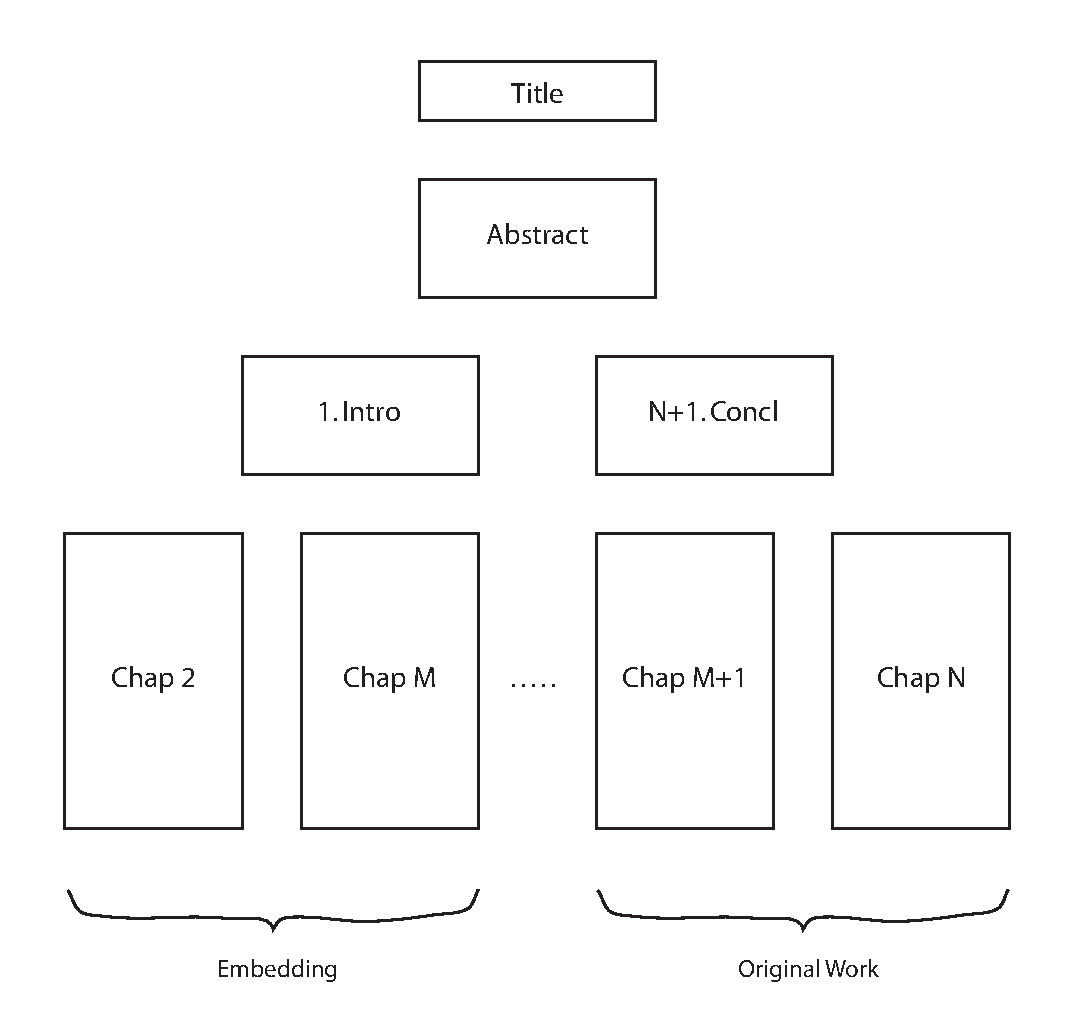
\includegraphics[keepaspectratio,width=\linewidth,height=\halfh]
{diagrams/pyramid.pdf}

\caption[Pyramid Writing Structure]{
Using a pyramid to structure a thesis into self-contained chunks
of increasing detail.
\imgcredit{Image drawn by the author of this thesis.}
}
\label{fig:Pyramid}
\end{figure}


The lesson from this is to structure your thesis as a pyramid in
self-contained units of increasing detail, as illustrated in
Figure~\ref{fig:Pyramid}. The main structural units are:
\begin{itemize}
\item \textbf{Title} \\
The title should be self-contained and comprise a good set of
representative keywords. Representative keywords in the title help
your work be found by an electronic search.

\item \textbf{Abstract} \\
The abstract should compactly, in two or three paragraphs, describe
the motivation for the work (embedding and context), what was done, and
the results and contributions (what is really new). As a rule of
thumb: the abstract summarises the thesis with about one sentence
corresponding to each chapter of the thesis.


\item \textbf{1. Introduction} \\
``Tell them what you are going to tell them''. As a rule of thumb: the
introduction contains one paragraph of text for each chapter in the
body of the thesis. Emphasise any original work and contributions.

\item \textbf{2. Embedding} \\
Two or three chapters embedding the thesis in the context of related
work, including an extensive literature survey.

\item \textbf{Chapter M}

\item \textbf{Chapter M+1} \\
Chapters containing the original work of the author.

\item \textbf{Chapter N}

\item \textbf{Concluding Remarks} \\
``Tell them what you told them''. One paragraph of text summarising
what was presented in each chapter of the body of the thesis.
Emphasise your own original work and achievements.

\item \textbf{Appendices} \\
Optional appendices might include a User Guide and a Developer
Guide, when software has been written as part of the thesis project.

\item \textbf{Bibliography} \\
There is some debate as to whether the bibliography should
be placed before or after any appendices. Many prefer after,
so that references can be looked up more easily. Others
prefer before, especially if there are extensive appendices.
If in doubt, ask your supervisor.

\end{itemize}




\section{Composing a Title and Abstract}

One useful strategy for composing a good title and abstract involves
brainstorming for a list of keywords. Start by writing down a list of
all the words and phrases describing important topics covered in the
thesis and which potential interested readers might use as search
terms to find the thesis. Then construct a title containing the most
important of these keywords. Finally, compose the abstract and make
sure most of the rest of the keywords are contained somewhere in the
abstract. Search engines and library systems will usually index the
title and the abstract, so anyone searching for any of the keywords
should now be able to find the thesis. When the thesis is approaching
completion, revisit the title and abstract, an extra extra keywords
and make any necessary adaptations.




\section{Double-Sided Printing}

Create and print your thesis in colour and for two-sided (duplex)
printing. Modern laser printers can easily handle printing out in
colour and double-sided. A thesis printed one-sided will be
(unnecessarily) twice as thick and twice as heavy.

Chapters, including the bibliography and any appendices, must
\emph{always} start on a new right-hand (odd-numbered) page.  This is
what the \lstinline!\cleardoublepage! command does.






\section{Single Children}

As in real life, a single child is not a good idea. A chapter with
only one section makes no sense. A section with only one subsection
makes no sense. A subsection with only one subsubsection makes no
sense either. If a structural unit has subunits, then there should
always be at least two subunits.







\section{Make Captions Carry the Story Too}

Some readers like to scan through your work from figure to figure,
gaining an impression of what it is about by reading the captions.
Support these readers by:
\begin{itemize}
\item \emph{Writing self-contained captions}: the caption
should describe the figure or table as completely as possible, without
assuming knowledge of material in the running text.

\item \emph{Writing longish captions}: it is fine for
captions to contain two or three sentences.

\item \emph{Stringing captions together}: Reading successive captions
should also tell an abridged version of the entire story.
\end{itemize}




\section{Avoid Orphan Floats}

Every floating element (figure, table, or listing) which appears in
the thesis and is given its own number such as Figure~3.1, Table~4.1,
or Listing~5.1 \emph{must} be discussed and referenced somewhere in
the running text. An orphan float is a float which appears and has a
number, but is never referenced in the flowing text.


          %   Chapter 3

\cleardoublepage
%----------------------------------------------------------------
%
%  File    :  thesis-academic.tex
%
%  Author  :  Keith Andrews, IICM, TU Graz, Austria
% 
%  Created :  27 May 93
% 
%  Changed :  19 Feb 2004
% 
%----------------------------------------------------------------


\chapter{Academic Writing}

\label{chap:Academic}


\chapquote{
Imitation is the sincerest flattery.
}
{
Charles Caleb Colton, English writer, 1780--1832.
}



Writing in an academic context is different to other types of
writing. Care must be taken to follow the conventions of
academic writing.



\section{Academic Criteria}

An academic thesis must demonstrate the following components:
\begin{itemize}
\item Motivation. What problem is being addressed and why.

\item Literature survey. A thorough review of related work in the field.

\item Original work. The original work of the author, and what is new
  about it.

\item An extensive bibliography. To demonstrate knowledge of the major
  works in the field, even if they have not all been read in their
  entirety.
\end{itemize}
Probably the most important component is to emphasise and underline
the author's own original contribution, i.e.\ how the work has
contributed to advancing the field.



\section{Academic Integrity}

It is very easy to find helpful material on the web. Resist the
temptation to copy such material verbatim, even with minor changes in
phrasing and word order. It is just as easy for a supervisor or
advisor (or anyone else for that matter) to check the originality of a
piece of text by copying a passage into Google or services such as
\parencite{PlagiarismOrg}.

Work submitted for academic assessment must be original and created by
the stated author(s). Care must be taken to avoid both
\emph{plagiarism} and \emph{breach of copyright}:
\begin{itemize}
\item \liintro{Plagiarism}: Using the work of others \emph{without
  acknowledgement}.

\item \liintro{Breach of copyright}: Using the work of others
  \emph{without permission}.
\end{itemize}





\subsection{Plagiarism}

Plagiarism is a violation of intellectual honesty. This means copying
other people's work or ideas without due acknowledgement, thus giving
the reader the impression that these are original (your own) work and
ideas. The Concise Oxford Dictionary, 8th Edition, defines plagiarism
as:
\begin{displayquote}
\enquote{
\textbf{plagiarise}
\textbf{1} take and use (the thoughts, writings, inventions, etc.\ of
another person) as one's own. \textbf{2} pass off the thoughts etc.\
of (another person) as one's own.
}
\end{displayquote}
Plagiarism is the most serious violation of academic integrity and can
have dire consequences, including suspension and expulsion
\parencite{Reisman2005}.



\subsection{Breach of Copyright}

Copyright law\footnote{Disclaimer: I am not a lawyer. The comments
  here reflect the situation to the best of my knowledge at the time
  of writing, but do not constitute legal advice. Laws sometimes
  change and I make no guarantees.} varies in detail from country to
country, but certain aspects are internationally widely accepted. In
general, the creator of a work, say a piece of writing, a diagram, a
photograph, or a screenshot, automatically has copyright of that
work. Copyright usually expires 70 years after the creator's
death. The copyright holder can grant the right for others to use or
publish their work on an exclusive or non-exclusive basis.

The copyright laws of most countries generally have provisions for
quoting small parts of a work. Austrian copyright law \parencite[§
  42f]{UrhG} allows for reasonable amounts of text to be quoted in
other works. It does not cover ``quoting'' entire images.




\section{Acceptable Use}

Academic work almost always builds upon the work of others, and it is
appropriate, indeed essential, that related and previous work by
others be discussed in an academic thesis. However, this must be done
according to the rules of acceptable use. There are two forms of
acceptable use:
\begin{itemize}
\item \liintro{Paraphrasing (Indirect Quotation)}: Summarising the ideas
  of someone else using original words and with attribution.
\item \liintro{Quoting (Direct Quotation)}: Including an exact
  verbatim copy inside quotation marks and with attribution.
\end{itemize}
Attribution means that the original source is cited.
Regardless of whether permission has been obtained from the copyright
owner or material is being used under the provisions of a specific
country's copyright law: whenever someone else's work is being used,
academic integrity dictates that the original source must be cited!
%
For further information on acceptable and non-acceptable academic
practice see \parencite{FremdeFedern,Wikipedia-Zitat}.




\subsection{Paraphrasing (Indirect Quotation)}

Paraphrasing means closely summarising and restating the ideas of
another person, but in (your own) original words. When writing a
literature survey, the relevant parts of each paper or source are
generally \emph{paraphrased}. One good technique for paraphrasing is:
\begin{enumerate}
\item Read the original source.
\item Put it down away from view.
\item \emph{Without refering to the original}, summarise it in your own words.
\end{enumerate}
When paraphrasing someone else's ideas, the original source must
always be cited!

Since paraphrased text is not enclosed in quotation marks, it is not
always obvious how to indicate the extent of the text which
corresponds to a particular citation. If the paraphrased text only
covers a single paragraph, include the citation either within or at
the end of the first sentence of the paragraph, or at the end of the
paragraph. Otherwise, describe the extent of the citation in words at
the beginning, for example: This section is based on the work of
\textcite{InfoSkyIVS}.





\subsection{Quoting Text (Direct Quotation)}

In some circumstances, it makes sense to directly \emph{quote} small
parts of text (typically a few sentences or paragraphs) from a
relevant source. When quoting directly, the \emph{exact} words,
spelling, and punctuation of the original are copied verbatim and
enclosed in quotation marks.

Most of an academic paper or thesis must be in words written by the
author(s) themselves. However, when an exact phrase or specific
wording from another source is important, then a direct quotation
should be used. In any case, the original source must be cited!

Short pieces of text can be quotes inline using the \vname{textquote}
command. For example, \textcite{DataAnalysisChallenges} define visual
analytics as an: \textquote{iterative process that involves collecting
  information, data preprocessing, knowledge representation,
  interaction, and decision making.}
%
Longer pieces of quoted text should be put into a \vname{displayquote}
environment. For example, as \textcite[page~99]{HarInfoVis}
explains:
\begin{displayquote}
\enquote{
Information in Hyper-G may be structured both hierarchically into
so-called \emph{collections}, and by means of associative hyperlinks.
A special kind of collection called a \emph{cluster} groups logically
related or multilingual versions of documents. Every document and
collection must belong to at least one collection, but may belong to
several. Navigation may be performed down through the collection
hierarchy (the collection \enquote{hierarchy} is, strictly speaking, a
directed acyclic graph), access rights assigned on a
collection-by-collection basis, and the scope of searches restricted
to particular sets of collections. Collections may span multiple
Hyper-G servers, providing a unified view of distributed resources.

Links in Hyper-G are stored in a separate link database and are
bidirectional (directed, but may be followed backwards): both the
incoming \emph{and} outgoing hyperlinks of a document are always
known and available for visualisation. Furthermore, Hyper-G has fully
integrated search facilities including full text search with relevance
scores and some limited support for similarity measures between
documents.

All in all, the richness of the Hyper-G data model provides plenty of
scope upon which to base visualisations: hierarchical structure,
(bidirectional) hyperlinks, and search and retrieval facilities. The
Harmony client for Hyper-G exploits this richness to provide
tightly-coupled two- and three-dimensional visualisation and
navigational facilities help provide location feedback and alleviate
user disorientation.
}
\end{displayquote}





\subsection{Quoting Images}

It is common to want to include photographs, diagrams, or screenshots
taken from the internet or from another work, particularly when
surveying related work. By default, it must be assumed that such
images are covered by copyright and \emph{cannot} simply be used.
Explicit permission \emph{must} be obtained for each image.

Sometimes, permission is granted in advance by the owner in the form
of a licence, such as one of the Creative Commons licences
\parencite{CC-Licences}. Other times, permission can be obtained
directly from the owner by sending a friendly email request. Without
permission, the image \emph{cannot} be used.

Once copyright has expired (in general, 70 years after the death of
the creator), an image passes into the public domain. However, even if
a rare original historical work may technically be in the public
domain, the owner of such a work controls access to it, and has
copyright over any photographs or scans of the work which they create.


For diagrams, an alternative strategy is to redraw and possibly adapt
the diagram in a (vector graphics) drawing editor such as Adobe
Illustrator \parencite{Adobe-Illustrator} or Inkscape
\parencite{Inkscape}. The original source should be cited with wording
like ``Redrawn from Figure N of [\ldots].'' or ``Adapted from Figure N
of [\ldots].''.

For graphs and plots, it is often possible to reconstruct the graphic
from the original data using tools such as gnuplot \parencite{gnuplot}
or R \parencite{R-Project}. The original source should be cited with
wording similar to ``Created from the original data [\ldots] using XY
[\ldots].''.


For screenshots of software, it is sometimes possible to obtain the
original software, install it, and make new screenshots. If possible,
an original, local dataset should be used rather than the default (or
a provided) dataset, so that the resulting screenshots are
demonstrably new and unique.
%
In the case of an online tool (running locally in a web browser), a
local original dataset should be loaded if possible. At a minimum, the
default view should be changed, so the resulting screenshot is new and
unique.
%
In both cases, the source of the software should be cited with wording
similar to ``Screenshot of XY [\ldots] created by the author of this
thesis.''.







\subsection{Attribution and Permission}

In general terms, for material included wholesale from elsewhere, two
pieces of information must be clearly stated:
\begin{enumerate}
\item \liintro{Attribution}: The original source of the material must
  be cited.

\item \liintro{Permission}: The terms under which the material is
  being used must be explained. For example, give the \emph{exact}
  Creative Commons licence \parencite{CC-Licences}, state the
  \emph{exact} legal exemption, or state that permission has kindly
  been given by the named original author.
\end{enumerate}

Attribution and permission should be stated in two places:
\begin{itemize}
\item \liintro{Caption}: At the end of the caption of a figure
  or listing containing the material.

\item \liintro{Credits}: In the Credits section at the
  front of the thesis.
\end{itemize}

All this means, of course, that if a thesis is based upon this
skeleton \parencite{KeithThesis}, then the source and permission
should be stated at the appropriate place (in this case, in the
Credits section).







\section{References}

Modern \LaTeXe installations use BibLaTeX \parencite{BibLaTeX} and
Biber \parencite{Biber} to maintain and process references. Much of
the syntax and many of the conventions were carried over from the
original BibTeX \parencite{BibTeX} format, but BibTeX is now obsolete.

Typically, one or more \vname{.bib} files are prepared, containing one
entry for each original source or reference.
Listing~\ref{list:BibFile} shows four typical entries from a
\vname{.bib} file. The \vname{inproceedings} entry describes a paper
published in conference proceedings, the \vname{article} entry
describes a paper published in a journal, and the \vname{booklet}
entry is being used for internet resources and web sites
(\vname{booklet} has the advantage over \vname{online} that it has a
\vname{howpublished} field.). Every entry type and field type is
documented in the BibLaTeX manual \parencite{BibLaTeX}. The BibLaTeX
Cheat Sheet \parencite{Biblatex-Cheatsheet} provides a convenient
overview.


\begin{samepage}
\lstinputlisting[%
  float=tp,
  aboveskip=\floatsep,
  belowskip=\floatsep,
  xleftmargin=0cm,              % no extra margins for floats
  xrightmargin=0cm,             % no extra margins for floats
%
  language=biblatex,
  basicstyle=\footnotesize\ttfamily,
  frame=shadowbox,
  numbers=left,
  label=list:BibFile,
  caption={[Four Typical Entries from a \vname{.bib} File]%
Four typical entries from a \vname{.bib} file for use
with biblatex and biber.
An \vname{inproceedings} entry describes a paper published
in conference proceedings, an \vname{article} entry describes
a paper published in a journal, and a \vname{booklet} entry
is used for internet resources and web sites.
The \vname{doi} field gives
the DOI (digital object identifier) of the paper.},
]
{listings/some.bib}
\end{samepage}


Of particular note is the \vname{doi} field, which gives the DOI
(digital object identifier) of a paper. DOIs are for academic papers
what ISBNs are for books; a unique handle with which one can easily
find the original. Most publishers are now assigning DOIs to new
conference and journal papers and are working back in time to assign
them to previously published papers. Always give the DOI of a paper
where one is available. If a DOI exists but points to a subscription
site, and the paper is also freely available on the web (say at the
home page of an author), then use the \vname{url} field to give the
free URL as well. Do not redundantly give the same URL in the
\vname{url} field which the DOI itself resolves to.





\subsection{Cleaning Downloaded Bib Entries}

\begin{samepage}
\begin{lstlisting}[%
  float=tp,
  aboveskip=\floatsep,
  belowskip=\floatsep,
  xleftmargin=0cm,              % no extra margins for floats
  xrightmargin=0cm,             % no extra margins for floats
  language=biblatex,
  basicstyle=\footnotesize\ttfamily,
  frame=shadowbox,
  numbers=left,
  label=list:BibACMIEEE,
  caption={[Massaging Bib Entries from ACM and IEEE]%
Bib entries copied from the ACM Digital Library or the
IEEE Computer Society Digital Library contain useful information,
but cannot be used ``as-is''. They must be edited to conform
to biblatex and to these thesis guidelines.
},
]
% From the IEEE Computer Society DL:

@article{10.1109/INFOVIS.2005.7,
author = {Martin Wattenberg},
title = {Baby Names, Visualization, and Social Data Analysis},
journal = {infovis},
volume = {0},
year = {2005},
issn = {1522-404x},
pages = {1},
doi = {http://doi.ieeecomputersociety.org/10.1109/INFOVIS.2005.7},
publisher = {IEEE Computer Society},
address = {Los Alamitos, CA, USA},
}


% From the ACM DL:

@inproceedings{1106568,
 author = {Martin Wattenberg},
 title = {Baby Names, Visualization, and Social Data Analysis},
 booktitle = {INFOVIS '05: Proceedings of the Proceedings of the 2005 IEEE Symposium on Information Visualization},
 year = {2005},
 isbn = {0-7803-9464-x},
 pages = {1},
 doi = {http://dx.doi.org/10.1109/INFOVIS.2005.7},
 publisher = {IEEE Computer Society},
 address = {Washington, DC, USA},
 }


% Clean, edited version for Keith:

@inproceedings{WattenbergNames,
  author       = "Martin Wattenberg",
  title        = "Baby Names, Visualization, and Social Data Analysis",
  booktitle    = "Proc.\ {IEEE} Symposium on Information Visualization
                  (InfoVis 2005)",
  venue        = "Minneapolis, Minnesota, USA",
  organization = "{IEEE} Computer Society",
  isbn         = "078039464X",
  date         = "2005-10",
  pages        = "1--8",
  doi          = "10.1109/INFOVIS.2005.7",
  url          = "http://hint.fm/papers/final-baby-margin-nocomments.pdf",
}

\end{lstlisting}
\end{samepage}


When \vname{.bib} entries are downloaded or copied from the ACM
Digital Library, the IEEE Digital Library, or other onlibne sources,
they should \emph{not} be used as is. They generally need to be
cleaned up first and made consistent with BibLaTeX.
Listing~\ref{list:BibACMIEEE} shows typical BibTeX entries provided by
the ACM Digital Library and the IEEE Computer Society Digital Library.


To bring bib entries into line with biblatex and the examples shown in
Listing~\ref{list:BibFile}, the following should be addressed:
\begin{itemize}
\item The title of the paper should use capitalised main words.

\item Capitalisations in the title which need to be preserved (such as
  the R in VRwave) should be enclosed in curly brackets ({VRwave}).

\item The \vname{title} and \vname{booktitle} should use
  capitalised main words (not all lower case).

\item The \vname{edition} field is usually be a number in inverted
  commas, such as \verb|"2"|, instead of a word such as
  \verb|"Second"|.

\item The name of a conference should be rephrased, with the short
  form of the conference name in parentheses at the end (InfoVis
  2005).

\item Any \vname{year}, \vname{month}, and \vname{day}
  fields should be combined into a \vname{date} field.

\item For a conference paper, the first day of the conference
  should be used as the date of publication.

\item The location of a conference should be in the \vname{venue}
  field, not in the \vname{address} or \vname{location} field. The
  \vname{address} field is for the address of the publisher, but is
  often unnecessary.


\item Any minus signs must be removed from the ISBN number.
  Otherwise, the macro used in this skeleton for handling ISBNs and
  linking to Amazon will break.

\item Any initial \vname{http://doi.acm.org/} or
  \vname{http://doi.ieeecomputersociety.org/} must be removed from
  the DOI. They are \emph{not} part of the DOI.

\item If a free, unofficial version of a paper with a DOI is available
  at the web site of one of the authors, give this in the \vname{url}
  field.

\item Manually shorten any URL as much as possible: try selectively
  removing parameters after a question mark and try removing
  \vname{www} from the domain. Do \emph{not} use a URL shortening
  service like \website{bit.ly}, since there is no guarantee the
  service will be around long term. It is acceptable to use a URL
  shortening service maintained by the original site themselves, such
  as \website{youtu.be} for YouTube URLs.

\end{itemize}







\subsection{What to Reference}

The set of references should be balanced:
\begin{itemize}
\item Do not have largely web sites as references. A few web sites as
  references is fine, most references being web sites is (usually) not
  so good.

\item Do not have too many Wikipedia references. A few Wikipedia
  references is OK; more than a few is not. Wikipedia is a good
  \emph{starting} point for (further) academic research, it is not a
  good ending point for academic research.

\item Have plenty of academic conference and journal papers (with a
  DOI). Sometimes, both an academic paper and a project web site will
  be avilable -- reference both as separate entries.

\item Include some books (with an ISBN) if at all possible. Books
  still count in academic circles.
 
\item If you know or suspect who will be reviewing or marking your
  thesis or paper, make sure to include some of their references. The
  first thing many reviewers do is check to see if they appear in the
  bibliography.

\item No ghost references. Every reference in the bibliography should
  be cited somewhere in the text.

\end{itemize}






\subsection{Citing}

When a citation is included within flowing text:
\begin{itemize}
\item Distinguish between \emph{parenthetical} and \emph{textual}
  citations. Parenthetical citations are used at the end of a
  sentence. Textual citations are used to embed the authors' names in
  the current sentence. For example:

\begin{small}
\hspace{2\parindent}
\renewcommand{\arraystretch}{1.5}
\begin{tabular}{p{0.45\linewidth}p{0.45\linewidth}}
\lstinline|\parencite{InfoSkyIVS}|        & \parencite{InfoSkyIVS}. \\
\lstinline|As \textcite{InfoSkyIVS} say,| & As \textcite{InfoSkyIVS} say,
\end{tabular}
\end{small}



\item If one specific part in a long paper or book is being cited,
  always state the page number or page range in the citation:

\begin{small}
\hspace{2\parindent}
\renewcommand{\arraystretch}{1.5}
\begin{tabular}{p{0.45\linewidth}p{0.45\linewidth}}
\lstinline|\parencite[pages 173--174]{InfoSkyIVS}|        &
  \parencite[pages 173--174]{InfoSkyIVS}. \\
\lstinline|As \textcite[pages 173--174]{InfoSkyIVS} say,| &
  As \textcite[pages 173--174]{InfoSkyIVS} say,
\end{tabular}
\end{small}



\item Multiple sources can be combined into one citation
command:

\begin{small}
\hspace{2\parindent}
\renewcommand{\arraystretch}{1.5}
\begin{tabular}{p{0.45\linewidth}p{0.45\linewidth}}
\lstinline|\parencites{InfoSkyStudies}[pages 173--174]{InfoSkyIVS}| &
  \parencites{InfoSkyStudies}[pages 173--174]{InfoSkyIVS}. \\
\lstinline|As \textcites{InfoSkyStudies}[pages 173--174]{InfoSkyIVS} say,| &
  As \textcites{InfoSkyStudies}[pages 173--174]{InfoSkyIVS} say,
\end{tabular}
\end{small}


\end{itemize}


Here are two examples embedded into some running text. The InfoSky
\parencite{InfoSkyIVS} system combined both hierarchical visualisation
and placement by similarity.
\textcite[Chapter~7]{InteractiveDataVisualisation} categorise
visualisation techniques for multi-variate data according to the
graphical primitive used in the rendering: points, lines, and regions.






% TODO
% https://www.cs.ubc.ca/~tmm/courses/cheat.html



       %   Chapter 4

\cleardoublepage
%----------------------------------------------------------------
%
%  File    :  thesis-style.tex
%
%  Author  :  Keith Andrews, ISDS, TU Graz, Austria
% 
%  Created :  27 May 1993
% 
%  Changed :  05 Nov 2018
% 
%----------------------------------------------------------------


\chapter{Language and Writing Style}
\label{chap:Style}


\chapquote{
It is an old observation that the best writers sometimes disregard the
rules of rhetoric. When they do so, however, the reader will usually
find in the sentence some compensating merit, attained at the cost of
the violation.
}
{
William Strunk, Jr., The Elements of Style, 1918.
}


A comprehensive guide to writing British English is the New Oxford
Style Manual \parencite{NewOxfordStyleManual-3Ed}. The Economist Style
Guide \parencite{EconomistStyleGuide-12Ed} provides a compact indexed guide
to British English usage. \textcite{Zinsser-OnWritingWell-7Ed} is an
easy to read companion.

A comprehensive guide to writing American English is the Chicago
Manual of Style \parencite{ChicagoManualStyle-17Ed}.  The classic
compact reference for American English writing style and grammar is
\textcite{StrunkWhite-4Ed}. The original text is now available for
free online \parencite{Strunk-1Ed}. Another good free guide is
\textcite{NASAGuide}.

\textcite{Alley-CraftScientificWriting-4Ed} is a classic guide to
scientific writing. Other good ones include
\textcite{Booth-CraftResearch-4Ed} and
\textcite{Booth-CommunicatingScience-2Ed}.
%
\textcite{Zobel-WritingCompSci} and \textcite{BugsInWriting} are guides
specifically aimed at computer science students.
\textcite{Phillips-HowGetPhD} gives practical advice for PhD
students.
%
In 2017, Google made its internal Documentation Style Guide
public \parencite{GoogleStyleGuide}.


Sections~\ref{sec:Clear} and \ref{sec:Gender} of this chapter are
adapted from the ACM CHI'94 conference language and writing style
guidelines.



% TODO
% https://www.cs.ubc.ca/~tmm/writing.html






\section{Paragraphs}

Sentences should be grouped into paragraphs by topic. A new paragraph
introduces a (slight) variation in topic. Paragraphs should consist of
\emph{several} sentences. In general, short paragraphs of only one or
two sentences should be merged topically with neighbouring paragraphs.
%
In \LaTeX, paragraphs are separated by a blank line. Random newlines
({\smaller\verb|\newline|} or {\smaller\verb|\\|}) should \emph{never}
be strewn throughout your text.

% In LaTeX, use a single-line comment to merge two short, but
% topically connected, paragraphs into one paragraph.





\section{Some Basic Rules of English}

There are a few basic rules of English for academic writing, which are
broken regularly by my students, particularly if they are non-native
speakers of English. Here are some classic and often encountered
examples:

\begin{itemize}[itemsep=2ex]

\item \emph{Never} use I, we, or you.

Write in the passive voice (third person).

\begin{tabular}{lp{0.9\linewidth}}
\dthumb & You can do this in two ways.   \\
\uthumb & There are two ways this can be done.  \\
\end{tabular}



\item \emph{Never} use he or she, his or her.

Write in the passive voice (third person).

\begin{tabular}{lp{0.9\linewidth}}
\dthumb & The user speaks his thoughts out loud.   \\
\uthumb & The thoughts of the user are spoken out loud.  \\
\end{tabular}

See Section~\ref{sec:Gender} for many more examples.



\item Stick to a consistent dialect of English. Choose either
  British or American English and keep to it throughout the
  whole of your thesis.



\item Do \emph{not} use slang abbreviations such as ``it's'',
  ``doesn't'', or ``don't''.

Write the words out in full: ``it is'', ``does not'', and ``do not''.

\begin{tabular}{lp{0.9\linewidth}}
\dthumb & It's very simple to\ldots       \\
\uthumb & It is very simple to\ldots       \\
\end{tabular}



\item Do \emph{not} use abbreviations such as ``e.g.'' or
  ``i.e.''. 

Write the words out in full: ``for example'' and ``that is''.

\begin{tabular}{lp{0.9\linewidth}}
\dthumb & \ldots in a tree, e.g. the items\ldots        \\
\uthumb & \ldots in a tree, for example the items\ldots   \\
\end{tabular}



\item Do \emph{not} use slang such as ``a lot of''.

\begin{tabular}{lp{0.9\linewidth}}
\dthumb & There are a lot of features\ldots       \\
\uthumb & There are many features\ldots       \\
\end{tabular}



\item Do \emph{not} use slang such as ``OK'' or ``big''.

\begin{tabular}{lp{0.9\linewidth}}
\dthumb & \ldots are represented by big areas.    \\
\uthumb & \ldots are represented by large areas.  \\
\end{tabular}



\item Do \emph{not} use slang such as ``gets'' or ``got''.

Use ``becomes'' or ``obtains'', or use the passive voice (third
person).

\begin{tabular}{lp{0.9\linewidth}}
\dthumb & The radius gets increased\ldots       \\
\uthumb & The radius is increased\ldots         \\
\end{tabular}

\begin{tabular}{lp{0.9\linewidth}}
\dthumb & The user gets disoriented\ldots       \\
\uthumb & The user becomes disoriented\ldots    \\
\end{tabular}




\item \emph{Never} start a sentence with ``But''.

Use ``However,'' or ``Nevertheless,''. Or consider joining the
sentence to the previous sentence with a comma.

\begin{tabular}{lp{0.9\linewidth}}
\dthumb & But there are numerous possibilities\ldots       \\
\uthumb & However, there are numerous possibilities\ldots  \\
\end{tabular}



\item \emph{Never} start a sentence with ``Because''.

Use ``Since'', ``Owing to'', or ``Due to''. Or turn the two
halves of the sentence around.




\item \emph{Never} start a sentence with ``Also''. Also should
be placed in the middle of the sentence.

\begin{tabular}{lp{0.9\linewidth}}
\dthumb & Also the target users are considered. \\
\uthumb & The target users are also considered. \\
\end{tabular}



\item Do \emph{not} use ``that'' as a connecting word.

Use ``which''.

\begin{tabular}{lp{0.9\linewidth}}
\dthumb & \ldots a good solution that can be computed easily.  \\
\uthumb & \ldots a good solution which can be computed easily.  \\
\end{tabular}




\item Do \emph{not} write single-sentence paragraphs. 

Avoid writing two-sentence paragraphs. A paragraph should contain at
least three, if not more, sentences.


\end{itemize}



% rules on the use of a comma in lists
% http://en.wikipedia.org/wiki/Serial_comma







\section{English Usage}
\label{sec:EnglishUsage}

I see these mistakes time and time again. Please do not
let me read one of them in your work.



\begin{itemize}[itemsep=2ex]


\item ``allows to'' is not English.

\begin{tabular}{lp{0.9\linewidth}}
\dthumb & The prototype allows to arrange components\ldots \\
\uthumb & The prototype supports the arrangement of components\ldots \\[1ex]
\dthumb & The system allows to identify issues\ldots \\
\uthumb & Issues can be identified by the system\ldots \\
\end{tabular}

% they allow to achieve



\item ``enables to'' is not English.

\begin{tabular}{lp{0.9\linewidth}}
\dthumb & it enables to recognise meanings\ldots \\
\uthumb & it enables the recognition of meanings\ldots \\
\end{tabular}



\item ``per default'' is not English.

Use ``by default''.

\begin{tabular}{lp{0.9\linewidth}}
\dthumb & Per default, the cursor is red. \\
\uthumb & By default, the cursor is red. \\
\end{tabular}




\item ``As opposed to'' is not English.

Use ``In contrast to''.

\begin{tabular}{lp{0.9\linewidth}}
\dthumb & As opposed to C, Java is object-oriented. \\
\uthumb & In contrast to C, Java is object-oriented. \\
\end{tabular}







\item ``actual'' \neqsym ``current'' 

If you mean ``aktuell'' in German, you probably mean
``current'' in English.

\begin{tabular}{lp{0.9\linewidth}}
\dthumb & The actual selection is cancelled. \\
\uthumb & The current selection is cancelled. \\
\end{tabular}



\item ``sensible'' \neqsym ``sensitive'' 

If you mean ``sensibel'' in German, you probably mean
``sensitive'' in English.

\begin{tabular}{lp{0.9\linewidth}}
\dthumb & Store sensible data securely. \\
\uthumb & Store sensitive data securely. \\
\end{tabular}




\item ``according'' \neqsym ``corresponding'' 

\begin{tabular}{lp{0.9\linewidth}}
\dthumb & For each browser, an according package is created. \\
\uthumb & For each browser, a corresponding package is created. \\
\end{tabular}




\item ``adopt'' \neqsym ``adapt'' 

To ``adopt something'' means ``etwas übernehmen'' in German.
To ``adapt something'' means ``etwas anpassen'' in German.

\begin{tabular}{lp{0.9\linewidth}}
\dthumb & This convention was adapted to show\ldots \\
\uthumb & This convention was adopted to show\ldots \\[1ex]
\dthumb & The diagram was adopted by the author. \\
\uthumb & The diagram was adapted by the author. \\
\end{tabular}



% countable and uncountable nouns
% https://english.stackexchange.com/questions/9439/amount-vs-number-vs-quantity
% https://dictionary.cambridge.org/grammar/british-grammar/amount-of-number-of-or-quantity-of

\item ``amount'' versus ``number'' 

Use ``number'' for countable things.
Use ``amount'' for uncountable things.

\begin{tabular}{lp{0.9\linewidth}}
\dthumb & The amount of students\ldots \\
\uthumb & The number of students\ldots \\[1ex]
\dthumb & The number of time\ldots \\
\uthumb & The amount of time\ldots \\
\end{tabular}



\item ``many'' versus ``much'' 

Use ``many'' for countable things.
Use ``much'' for uncountable things.

\begin{tabular}{lp{0.9\linewidth}}
\dthumb & Much students failed\ldots \\
\uthumb & Many students failed\ldots \\[1ex]
\dthumb & Many time was spent\ldots \\
\uthumb & Much time was spent\ldots \\
\end{tabular}



\item ``fewer'' versus ``less'' 

Use ``fewer'' for countable things.
Use ``less'' for uncountable things.

\begin{tabular}{lp{0.9\linewidth}}
\dthumb & Less participants succeeded\ldots \\
\uthumb & Fewer participants succeeded\ldots \\[1ex]
\dthumb & Fewer sand was blown away\ldots \\
\uthumb & Less sand was blown away\ldots \\
\end{tabular}





\item ``\emph{anything}-dimensional'' is spelt with a hyphen.

For example: two-dimensional, three-dimensional.


\item ``\emph{anything}-based'' is spelt with a hyphen.

For example: tree-based, location-based.


\item ``\emph{anything}-oriented'' is spelt with a hyphen.

For example: object-oriented, display-oriented.


\item ``\emph{anything}-side'' is spelt with a hyphen.

For example: client-side, server-side.


\item ``\emph{anything}-friendly'' is spelt with a hyphen.

For example: user-friendly, customer-friendly.


\item ``\emph{anything}-to-use'' is spelt with hyphens.

For example: hard-to-use, easy-to-use.


\item ``\emph{anything}-level'' is spelt with a hyphen.

For example: low-level, high-level.



\item ``realtime'' is spelt with a hyphen if used as
  an adjective, or as two separate words if used as a noun.

\begin{tabular}{lp{0.9\linewidth}}
\dthumb & \ldots display the object in realtime.  \\
\uthumb & \ldots display the object in real time. \\
\dthumb & \ldots using realtime shadow casting.   \\
\uthumb & \ldots using real-time shadow casting.  \\
\end{tabular}


\end{itemize}












\section{Clear Writing}
\label{sec:Clear}

An academic thesis written in English should use simple and clear
language appropriate for an international audience. In particular:

\begin{itemize}[itemsep=2ex]

\item Write simple, straightforward sentences. Do not use long,
  convoluted sentences with many nested clauses, purely for the whim
  of it, because, as is sometimes the case, it may seem like a good
  idea at the time, even though it is not really.


\item Use common and basic vocabulary. For example:
  \begin{itemize}
  \item ``unusual'' instead of ``arcane''
  \item ``specialised'' instead of ``erudite''.
  \item ``guideline'' instead of ``rule of thumb''.
  \end{itemize}



\item A technical term should be defined once at first usage.  It
  should be placed in italics where it is defined, and in normal
  script whenever used thereafter:

\begin{tabular}{lp{0.9\linewidth}}
\uthumb & A \emph{graph} is a set of vertices and edges.
        A \emph{vertex} (or node) is an individual item. \newline
        An \emph{edge} (or link) is a connection between two vertices.
\end{tabular}

  Any equivalent variant terms should be listed with the
  definition. The preferred term should then be used consistently
  throughout the text, rather than any of the variant terms.
  Otherwise, readers are left wondering whether the variant term
  refers to the same thing or is something different.



\item For generic English text, rather than repeating the same word or
  phrase too often, look in a thesaurus (see
  Section~\ref{sec:thesaurus}) for an alternative word with the same
  meaning.


\item Explain any acronyms the first time they are used, by writing
  out the full phrase followed by the acronym in parentheses.

\begin{tabular}{lp{0.9\linewidth}}
\dthumb & When using SVG, the figure scales freely. \\
\uthumb & When using Scalable Vector Graphics (SVG), the figure scales freely.
\end{tabular}


\item Avoid local references. International readers will probably not
  recognise the names of the provincial capitals of Austria, for
  example. If local context is necessary for understanding, then
  describe it fully.


\item Avoid ``insider'' jargon. Do not assume knowledge of a
  particular context. For example, do not assume the reader is
  familiar with a particular operating system or application.


\item Express culturally localised things such as times, dates,
  currencies, and numbers in an unambiguous form. For example, 9/11 is
  the \nth{9} of November in much of the world. In English, a period
  ``.''  is used as the decimal point character and a comma ``,'' is
  used as the thousands separator (in German, it is the other way
  round).


\item Do not use ``word plays'' or puns. Phrases such as ``red
  herring'', ``taking the mickey'', and ``like watching paint dry''
  require cultural knowledge of English to understand.


\item Be careful with humour. Irony and sarcasm are sometimes hard to
  detect for non-native speakers.

\end{itemize}


Part of writing usable documents is understanding and then addressing
the characteristics of the intended audience.





\section{Avoiding Gender Bias}
\label{sec:Gender}

Two issues should be considered with regard to avoiding gender bias:
avoiding characterisations or stereotypes about men or women,
and avoiding biases inherent in the English language.
Here are some suggestions for handling the second issue:

\begin{itemize}[itemsep=2ex]

\item Refer to people generically using a gender-neutral term:

\begin{tabular}{ll}
   man                 &   the human race        \\
   mankind             &   humankind, people     \\
   manpower            &   workforce, personnel  \\
   man on the street   &   average person        \\
\end{tabular}



\item Use gender-neutral terms for job titles or roles, where
  possible:

\begin{tabular}{ll}
  chairman     &  chairperson \\
  spokesman    &  spokesperson, representative \\
  policeman    &  police officer \\
  stewardess   &  flight attendant \\
\end{tabular}



\item When refering to the holder of a specific position and their
  gender is known, use the correct gender pronoun. For example,
  assuming the chairperson is known to be a man:

\begin{tabular}{lp{0.9\linewidth}}
\dthumb & The chairperson announced her resignation. \\
\uthumb & The chairperson announced his resignation. \\
\end{tabular}



\item Avoid using a gender pronoun by repeating the job title or role
  if possible:

\begin{tabular}{lp{0.9\linewidth}}
\dthumb&
Interview the user first and then ask him to fill out a questionnaire. \\
%
\uthumb &
Interview the user first and then ask the user to fill out a questionnaire. \\
\end{tabular}



\item Avoid using his or her by using the plural form:

\begin{tabular}{lp{0.9\linewidth}}
\dthumb & Each student should bring his text to class. \\
\uthumb & All students should bring their texts to class. \\
\end{tabular}


\item Replace his or her with the article (the):

\begin{tabular}{lp{0.9\linewidth}}
\dthumb & Every student must hand his report in on Friday. \\
\uthumb & Every student must hand the report in on Friday. \\
\end{tabular}



\item Avoid using his or her by rewriting in the passive voice:

\begin{tabular}{lp{0.9\linewidth}}
\dthumb & Each department head should do his own projections. \\
\uthumb & Projections should be done by each department head. \\
\end{tabular}


\item Avoid awkward formulations such as ``s/he,'' ``he/she,'' or
  ``his/her.'' As a last resort, use the less awkward ``he or she,''
  or ``his or hers.''

\end{itemize}






\section{When to Use Capitalisation}

\emph{Capitalisation} means using a capital (upper case) initial
letter for a word. \emph{Lowercasing} means writing the entire word in
lower case. In many common writing styles, headings and titles are
partially capitalised: the first and the principal (main) words are
capitalised and other words are lowercased.

Proper names, such as the names of people, towns, and countries, are
always capitalised (Keith Andrews, the United Kingdom). The first word
in a heading or title is always capitalised.




\subsection{Titles and Headings}

Capitalise all principal words: nouns, pronouns, adjectives, verbs,
and adverbs, and the first word. Lowercase all articles, coordinating
conjunctions (``for'', ``and'', ``nor'', ``but'', ``or'', ``yet'',
``so''), and prepositions.

For example:
\begin{itemize}[itemsep=2ex]

\item Here, ``it'' is a pronoun, which should always be capitalised.

\begin{tabular}{lp{0.9\linewidth}}
\dthumb & Saying it Directly \\
\uthumb & Saying It Directly \\
\end{tabular}



\item Here, ``is'' is a verb, which should always be capitalised.

\begin{tabular}{lp{0.9\linewidth}}
\dthumb & When is Enough Enough? \\
\uthumb & When Is Enough Enough? \\
\end{tabular}



\item Here, ``in'' is being used as a preposition and should be 
lowercased.

\begin{tabular}{lp{0.9\linewidth}}
\dthumb & The Elephant In the Room. \\
\uthumb & The Elephant in the Room. \\
\end{tabular}


\item Here, ``in'' is being used as an adverb and should be 
capitalised.

\begin{tabular}{lp{0.9\linewidth}}
\dthumb & Handing in Your Work. \\
\uthumb & Handing In Your Work. \\
\end{tabular}


\end{itemize}

See \textcite{WB-Capitalisation} for some slightly different rules and
some more examples.


% Capitalization in Titles
% http://www.writersblock.ca/tips/monthtip/tipmar98.htm




\subsection{Captions}

The short version (the optional parameter in square brackets) of a
caption for a figure, table, or listing appears in the List of
Figures, List of Tables, or List of Listings. The short caption is
used like a heading and should be capitalised like a heading. The long
version of a caption for a figure, table, or listing should be written
as full sentences: only the first word of each sentence and any proper
names are capitalised and (each sentence in) the caption ends with a
full stop.



\subsection{Chapters, Sections, Figures, and Tables}

A specific, named or numbered entity, such as a particular chapter,
appendix, section, figure, table, or listing is considered to be a
proper name and thus \emph{should be capitalised}. For example,
Chapter~\ref{chap:SelectedDetails}, Appendix~\ref{app:UserGuide},
Section~\ref{sec:Gender}, Figure~\ref{fig:TeXnicCenter},
Table~\ref{tab:WinIconicLang}, or Listing~\ref{list:BibFile}. However,
if an entity is not specifically named or numbered, then it should
\emph{not} be capitalised. For example, when refering to the first
chapter or the next section, without giving a name or number.


% Capitalization Rules
% http://www.libraryonline.com/default.asp?pID=48

% Chicago Manual of Style
% http://www.chicagomanualofstyle.org/home.html

% Associated Press Stylebook
% http://www.apstylebook.com/







\section{Use a Spelling Checker}

In these days of high technology, spelling mistakes and typos are
inexcusable. It is \emph{very} irritating for your supervisor to have
to read through and correct spelling mistake after spelling mistake
which could have been caught by an automated spelling checker.
Believe me, irritating your supervisor is not a good idea.

So, use a spelling checker \emph{before} you hand in \emph{any}
version, whether it is a draft or a final version.
Since this is apparently often forgotten, and sometimes even wilfully
ignored, let me make it absolutely clear:
\begin{quote}
\begin{em}
Use a spelling checker, please. \\
Use a spelling checker! \\
Use a spelling checker, you moron. \\
\end{em}
\end{quote}





\section{Use a Dictionary}
\label{sec:dictionary}

If you are not quite sure of the meaning of a word, then use a
dictionary. \website{dictionary.com} \parencite{DictionaryCom} is a
free English dictionary, BEOLINGUS \parencite{DictChemnitz} and Leo
\parencite{DictLeoOrg} are two very good English-German dictionaries.




\section{Use a Thesaurus}
\label{sec:thesaurus}

If a word has been used several times already, and using another
equivalent word might improve the readability of the text, then
consult a thesaurus. \website{thesaurus.com} \parencite{ThesaurusCom}
and Collins English Thesaurus \parencite{CollinsThesaurus} are free
English thesauri.


          %   Chapter 5

\cleardoublepage
\chapter{Giving a Presentation}

\label{chap:Presentation}

  %   Chapter 6

% ....


% Part 2 Original Work

\cleardoublepage
\chapter{Technical Realisation}

\label{chap:Tech}
           %   Chapter N

\cleardoublepage
%----------------------------------------------------------------
%
%  File    :  thesis-details.tex
%
%  Author  :  Keith Andrews, IICM, TU Graz, Austria
% 
%  Created :  17 Nov 2004
% 
%  Changed :  17 Nov 2004
% 
%----------------------------------------------------------------

\chapter{Selected Details of the Implementation
(and Test of Extremely
Long Chapter Titles to See How They Work or Not)
}

\label{chap:SelectedDetails}


\chapquote{
The devil is in the detail.
}
{
English proverb.
}


There are often specific details of a project, which involve
particularly much work to get right, but do not form a major part in
the whole scheme of things, so would not generally deserve a chapter
of their own. This chapter is for these details.



\section{First Selected Detail}

The context, the decision process, all the variations that were tried,
and the solution that was finally adopted.



\section{Second Selected Detail}

From some other part of the project. Explaining your reasoning and
choices will help some other poor student, who has to pick up your
work from where you left off.



\section{Using a Table}

An example of using a table can be seen in Table~\ref{tab:BestPubs}.

\begin{table}[tp]
\centering
\begin{tabularx}{\linewidth}{|llrX|}
\hline
Name & Type & Rating & Description \\
\hline
Flann O'Brien &
Irish &
***** &
In the centre of town and easy to find for
marauding tourists. Very smooth Guinness.
\\
\hline
The Office &
English &
***** &
Hidden in the narrow streets of the old town.
Erasmus student night every other Wednesday.
\\
\hline
O'Carolans &
Irish &
*** &
In the centre of town in a small side street next to Flann's.
Small, cosy, but hellishly smoky.
\\
\hline
O'Riginal &
pseudo Irish &
 &
Austrian dive pretending to be an Irish pub.
\\
\hline
\end{tabularx}

\caption[Best Pubs in Graz]
{
The best pubs in Graz.
}
\label{tab:BestPubs}
\end{table}





\section{Using Subfigures}

This example shows how to include vector graphics in the form of PDF
files. It also shows how to use subfigures within a figure.

\begin{figure}[tp]
\centering
\subfloat[][%  the % chars remove implicit spacing
An object has been composed to represent an
abstract version of the clock tower in Graz.
Here, the object is in its initial state.
]
{%
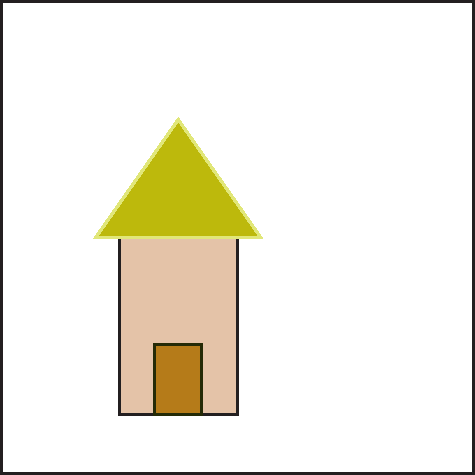
\includegraphics[width=0.45\linewidth]
{diagrams/multi1.pdf}%
\label{fig:Tower1}%
}
\hfill
\subfloat[][%
The object has been scaled and rotated, and now resembles
a leaning tower.
]
{%
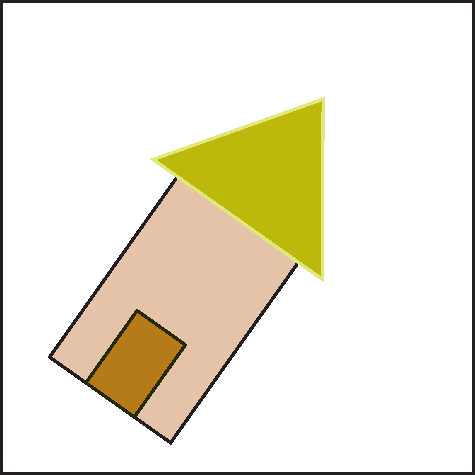
\includegraphics[width=0.45\linewidth]
{diagrams/multi2.pdf}%
\label{fig:Tower2}%
}

\caption[Abstract Clock Towers]
{
The leaning tower of Graz. An abstract model of the clock
tower in Graz leaning over time. \subref{fig:Tower1} shows
the initial state. \subref{fig:Tower2} shows the final state.
\imgcredit{Both images created by the author of this thesis.}
}
\label{fig:WholeFig}
\end{figure}


An example of using the \vname{subfig} package can be seen in
Figure~\ref{fig:WholeFig}. Figure~\ref{fig:Tower1} shows the polygons
before transformation, while Figure~\ref{fig:Tower2} shows them
afterwards.





\section{Including a Screenshot}

This example shows how to include a screenshot (or other raster
graphic) into a \LaTeXe\ figure.

\begin{figure}[tp]
\centering
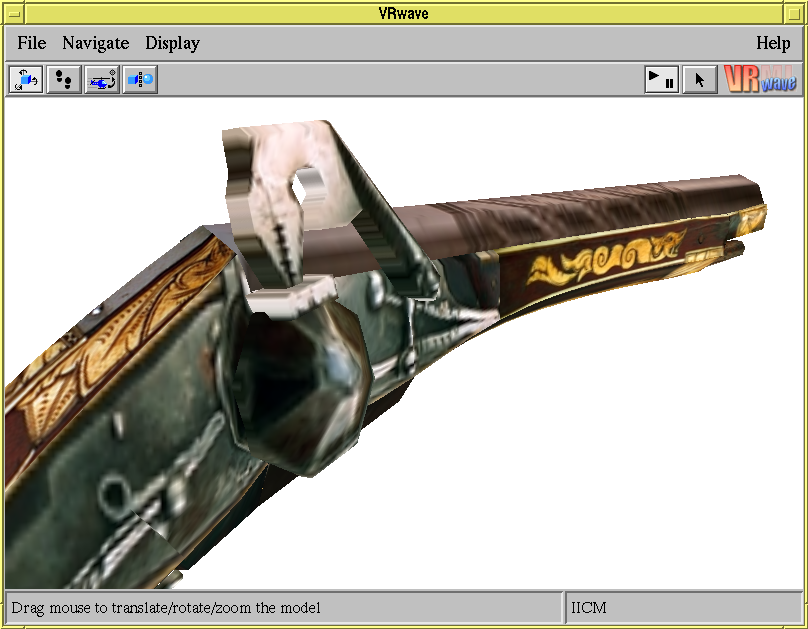
\includegraphics[keepaspectratio,width=\linewidth,height=\halfh]
{images/pist.png}

\caption[VRwave in Flip Mode]
{%
VRwave in Flip mode displaying a textured model of a cavalry pistol
from the world-renowned Zeughaus (armoury) in Graz.
\imgcredit{Image extracted from \textcite[page~81]{Andrews-VRwave}
and used under the terms of the ACM Copyright Policy. \copyrightACM}
}
\label{fig:Pistol}
\end{figure}


An example of how to correctly cite the source when using an image
from someone else. In their 1998 paper, \textcite{Andrews-VRwave}
discuss the VRwave VRML browser. Figure~\ref{fig:Pistol} shows a VRML
model of a cavalry pistol from the Armoury in Graz displayed in the
VRwave VRML browser.





\section{Using Special Characters and Symbols}

You can use many (but not all) of the thousands of characters
available in the UTF-8 \parencites{Wikipedia-UTF8}{Unicode-Charts}
character encoding. For example, the German umlauts (äüö), the German
sharp s (ß), or the yen symbol (¥).

You can also try some of the \approxsym 100 symbols available
in the \vname{textcomp} package, such as the yen symbol (\textyen) and
a circled letter A (\textcircled{A}).



\section{Using Macros to Style Special Names}

Use the \vname{vname}, \vname{cname}, and \vname{fname} macros to
define the style for (say) variable names, class names, and file
names. You can also define your own macros. The is a very long file
name \fname{/usr/data/keith/travel/austria/vienna.txt} to see how they
are broken at a line end. A typical class name is
\cname{HVSInformationPyramidsInputFactory}.





\section{Using Macros as Shorthand}

Sometimes, a macro (new command definition) can be useful to define
the contents of table cells, particularly if these contain images. For
example, Table~\ref{tab:WinIconicLang} uses the macro called
\vname{iibox}, which takes a single parameter, the name of
the particular image.


\begin{table}[tp]

\newcommand{\iibox}[1]{\parbox[c][1cm][c]{1cm}{%
\includegraphics[scale=0.6]{./images/icons/#1.png}
}}

\begin{center}
\begin{tabular}[t]{|p{7cm}c|}
\hline
\multicolumn{2}{|l|}{\sffamily \bfseries Elementary Symbols}            \\
Document                            & \iibox{win-il-gen-doc}            \\
Assistant                           & \iibox{win-il-gen-ass}            \\
Template                            & \iibox{win-il-gen-tmpl}           \\
\hline
\multicolumn{2}{|l|}{\sffamily \bfseries Document Types}                \\
Text document                       & \iibox{win-il-text-doc}           \\
Spreadsheet document                & \iibox{win-il-spreadsheet-doc}    \\
Presentation document               & \iibox{win-il-presentation-doc}   \\
Database document                   & \iibox{win-il-database-doc}       \\
\hline
\multicolumn{2}{|l|}{\sffamily \bfseries Applications}                  \\
Word                                & \iibox{win-il-word-appl}          \\
Excel                               & \iibox{win-il-xls-appl}           \\
Powerpoint                          & \iibox{win-il-ppt-appl}           \\
Access                              & \iibox{win-il-mdb-appl}           \\
\hline
\multicolumn{2}{|l|}{\sffamily \bfseries Generated Icons}               \\
Word text document                  & \iibox{win-il-word-doc}           \\
Excel spreadsheet document          & \iibox{win-il-xls-doc}            \\
Powerpoint presentation document    & \iibox{win-il-ppt-doc}            \\
Access database document            & \iibox{win-il-mdb-doc}            \\[2ex]
%
Word template                       & \iibox{win-il-word-tmpl}          \\
Powerpoint template                 & \iibox{win-il-ppt-tmpl}           \\
Access template                     & \iibox{win-il-mdb-tmpl}           \\[2ex]
%
Word template assistant             & \iibox{win-il-word-ass}           \\
Powerpoint template assistant       & \iibox{win-il-ppt-ass}            \\
Access template assistant           & \iibox{win-il-mdb-ass}            \\[2ex]
%
\hline
\end{tabular}
\end{center}

\caption[Iconic language for Windows NT 4.0 documents]
{
Iconic language for Windows NT 4.0 documents.
\imgcredit{The icons are screenshots, captured and then
enlarged by the author of this thesis.}
}
\label{tab:WinIconicLang}
\end{table}







\begin{samepage}
\begin{lstlisting}[%
  float=tp,
  aboveskip=\floatsep,
  belowskip=\floatsep,
  xleftmargin=0cm,              % no extra margins for floats
  xrightmargin=0cm,             % no extra margins for floats
  basicstyle=\footnotesize\ttfamily,
  frame=shadowbox,
  numbers=left,
  language=HTML,
  label=list:HTML5Boilerplate,
  caption={[HTML5 Boilerplate Code]%
Some HTML5 boilerplate code, illustrating the typical structure
of a HTML5 web page.
},
]
<!DOCTYPE html>
<html xmlns="http://www.w3.org/1999/xhtml" lang="en" xml:lang="en">

<head>
<meta charset="UTF-8"/>
<meta name="viewport" content="width=device-width, initial-scale=1"/>
<link rel="stylesheet" href="./inm.css"/>

<title>Keith Andrews Web Page</title>
</head>

<body>

<header>
<img src="images/kalogo.svg" alt="KA Logo"/>
Keith Andrews Design
</header>

<h1>Keith Andrews</h1>

<p>
Keith lives in <a href="http://graz.at/">Graz</a>.
</p>

<p>
<img src="images/keith-s.jpg"
  alt="Photo of Keith Andrews"/>
</p>

<p>
Three desirable attributes:
</p>
<ol>
<li>cheap</li>
<li>fast</li>
<li>good</li>
</ol>
<p>
Choose any two.
</p>

<p>
<abbr title="Extensible HyperText Markup Language">XHTML</abbr>
is cool.
</p>

<table>
<tbody>
<tr><th>Beer</th><th>Price €</th></tr>
<tr><td>Puntigamer</td><td>2,60</td></tr>
<tr><td>Gösser</td><td>2,60</td></tr>
<tr><td>Guinness</td><td>4,35</td></tr>
</tbody>
</table>

<footer>
Copyright © Keith Andrews 2019.
</footer>

</body>
</html>
\end{lstlisting}
\end{samepage}



\section{Using Floating Listings}

Listing~\ref{list:HTML5Boilerplate} is floating. A floating listing is
a block of code treated like other \LaTeXe floats (such as figures or
tables). Use floating listings for longer blocks of code.
A floating listing is given a number and can be referred to
explicitly, like Listing~\ref{list:HTML5Boilerplate}. It can be given
a caption and short caption, and is listed in the List of Listings.





\section{Using Non-Floating Diplayed Listings}

The listing below shows some CSS:
\begin{samepage}
\begin{lstlisting}[%
  language=CSS,
]
body { color: black; background-color: silver; }
img { border: none; }
h1,h2 { font-family: Verdana, sans-serif; }
\end{lstlisting}
\end{samepage}
It is displayed (i.e. indented as a block) in-place, but is not
floating. It cannot be referred to by number and is not listed in the
List of Listings. As a rule of thumb, if listings have five or more
lines, make them floating.





\section{Using Inline Listings}

Inline listings are used for very short snippets of code embedded
within the flow of a paragraph. For example,
\lstinline|\lstinline!var i:integer;!|
produces
\lstinline!var i:integer;!, which can now be discussed further.
Do not break an inline listing over multiple lines (EOL).




\section{Using Lists}

A list should always be introduced by a sentence
which ends with a colon.
%
There are three kinds of standard lists in \LaTeXe:
\begin{itemize}
\item itemize
\item enumerate
\item description
\end{itemize}
% A blank line here would indicate a new (indented) paragraph
An enumerated list has numbered items:
\begin{enumerate}
\item Fast
\item Good
\item Cheap
\end{enumerate}
Choose any two!


A description list has named items with corresponding
definitions or descriptions:
\begin{description}
\item[Short] Each item has a label (name) and its description.

\item[Rather longer label] By default, if the description text
  is rather long, it will warp around to the following lines.
\end{description}



        %   Selected Details

\cleardoublepage
\chapter{Outlook and Future Work}
\label{chap:Outlook}

Many things could still be done to the RespVis library that would not
change its core mechanisms, but would improve both the visualization
consumer's and visualization author's experience. One of the most
apparent improvements would be the addition of further Series, Charts,
and Chart Windows to extend the range of realizable visualizations and
enable the creation of things like parallel coordinates, pie charts,
heatmaps, small multiples, and other charts. In addition to supporting
more types of charts, the RespVis library would benefit from
additional tools which could be added to the Toolbars of Chart Windows
to provide easy access to supplementary operations like interval-based
numerical filtering and zooming. The improvements that could be made
to already existing functionality include improving interactions via
the application of Delaunay triangulation
\parencite{Delaunay,DelaunayAlgorithms} to find the closest
interactable element to the cursor position, improving downloaded SVGs
through optimizing and formatting their document contents, and
improving responsive styling via the application of the newly proposed
CSS Container Queries \parencite{CSSContainment3} when they become
available in browsers.

The layouting of SVG elements could be improved by separating
visualizations into different <div> elements that can be natively laid
out by browsers. With such a layouting mechanism, the custom Layouter
could be removed, and the render process imposed by it, which
effectively forces every laid out element to be rendered twice, would
be unnecessary. The elimination of the custom Layouter and its render
process would improve performance and be much less complex to
implement and understand. The downside of this change would be that
visualizations are not directly rendered as pure and complete SVG
documents anymore, but rather as multiple SVG documents representing
separate parts of the visualization. This separation into multiple SVG
documents would not be a problem for displaying visualizations in
browsers. To download such a visualization, its individual parts could
be merged back into a pure and complete SVG document during an
additional download pre-processing step.

Custom visualizations are rather tedious to create with the current
implementation, because visualization authors must manually set up
their structure, propagate data through the component hierarchy, and
handle the Layouter's render process. The creation of custom
visualizations could be simplified by introducing generic Chart
Windows that would enable the definition of visualizations using a
data structure potentially similar to visualization grammars like Vega
\parencite{Vega}.
% KA TODO or Cicero or Vega-Lite ??
The data structure of generic Chart Windows would have to include the
actual abstract data that should be visualized and define the
transformations of this data into scales, Axes, Legends, and Series.
During rendering, the render functions of such generic Chart Windows
could then create custom visualizations to reflect the configuration
stored in these data structures. In addition to simplifying the
creation of custom visualizations, generic Chart Windows would also
enable responsively changing a visualization's encoding, like, for
example, turning Point Charts into Heatmap Charts.


% KA TODO  small multiples?



        %   Outlook

\cleardoublepage
\chapter{Concluding Remarks}
\label{chap:Concl}

After giving an overview of related web technologies and the research related to the academic fields of information visualizations and responsive visualizations, this thesis introduced RespVis, a new open-source software library to create responsive visualizations for the web.
RespVis has been designed as an extension of the D3 library and renders visualizations as SVG documents styled with CSS.
The most novel contribution of this work is a custom layouter that uses the browser's own layout engine to enable visualization authors to configure the layout of SVG-based visualization components via CSS.
Since rearranging content is one of the main techniques of responsive web design, enabling visualization authors to use CSS layout mechanisms like Flexbox and Grid to reposition visualization components leads to much better responsive capabilities than merely allowing them to change their styles.
Relying on CSS for a large amount of a visualization's configuration also leads to visualization authors benefitting from being able to utilize CSS media queries for responsive styling and from the simplicity of using a tool they are already familiar with.
Furthermore, since RespVis' API is mostly meant for configuring a visualization's content and behavior, it can be much more minimal than it would be if the complete style of a visualization would also be configured via it.
This minimal API and RespVis' reliance on standards like SVG and CSS for rendering and configuring its visualizations result in much less likelihood that visualization authors are limited by API restrictions.
Due to all of these reasons, it is evident that RespVis has the potential to be a very effective library for the creation of responsive visualizations after some more improvements are made to it.
          % Concluding Remarks



\appendix

\cleardoublepage
%----------------------------------------------------------------
%
%  File    :  thesis-user.tex
%
%  Author  :  Keith Andrews, ISDS, Graz University of Technology
% 
%  Created :  27 Jan 2019
% 
%  Changed :  27 Jan 2019
% 
%----------------------------------------------------------------

\chapter{User Guide}

\label{app:UserGuide}

A thesis in computer science will often involve the writing of
software. In such cases, it is common to have a user guide and
sometimes also a developer guide as appendices.
The user guide is aimed at end users of the software.
It typically covers the following aspects:
\begin{itemize}
\item \liintro{Installation}: a description of how to install the
  software.

\item \liintro{Features}: an overview of what the software can do.

\item \liintro{User Interface}: a thorough tour of elements of the
  user interface, their purpose, and how to use them, illustrated with
  numerous screenshots.

\item \liintro{Usage}: a series of ``recipes'' explaining how to
  accomplish common tasks.

\item \liintro{FAQs}: answers to a number of (anticipated) frequently
  asked questions.
\end{itemize}
The user guide should be a stand-alone document, complete in itself,
even if that requires some duplication with material or screenshots
contained within the main thesis.


           % Appendix A

\cleardoublepage
%----------------------------------------------------------------
%
%  File    :  thesis-developer.tex
%
%  Author  :  Keith Andrews, ISDS, Graz University of Technology
% 
%  Created :  27 Jan 2019
% 
%  Changed :  27 Jan 2019
% 
%----------------------------------------------------------------


\chapter{Developer Guide}
\label{app:DeveloperGuide}

The developer guide is aimed at fellow developers, who might modify or
extend the software in future. It typically covers some or all of the
following aspects:
\begin{itemize}
\item Development environment and tools.

\item Software dependencies.

\item APIs.

\item Mechanisms for extensions, such as hooks or plugins.

\item How to integrate a new piece of code, such as an
  alternative search algorithm or visualisation.
\end{itemize}



      % Appendix B



\backmatter

% Ensure that certain references are listed in the bibliography,
% even if they are not cited anywhere in the text.
% \nocite{KeithMastersThesis}
% \nocite{KeithPhdThesis}


\cleardoublepage
% for now, switch to language english
% hack to force unix date for biblio, biblatex 3.11
\begin{otherlanguage}{english}
\printbibliography[heading=bibintoc]
\end{otherlanguage}



% \cleardoublepage
% \input{glossary}      % Glossary
 
% \cleardoublepage
% \input{index}         % Index

\end{document}

